\documentclass[12pt,onecolumn,a4paper,twoside,final]{article}
\usepackage{graphicx}
\usepackage[margin=5pt]{subcaption}
\usepackage{fullpage}
\usepackage{cite}
\usepackage{hyperref}
\usepackage{booktabs}
\usepackage{tabularx}
\usepackage{lipsum}
\usepackage{siunitx}
\usepackage{float}
\usepackage{multicol}
\usepackage{pdfpages}
\usepackage{amsfonts}
\usepackage{amsmath}
\usepackage{listings}
\usepackage[toc,page]{appendix}

\graphicspath{ {fig/} }
\captionsetup{format=hang}

\setlength{\parindent}{0pt}

\begin{document}

%% LIS Report Header Template
%%%%%%%%%%%%%%%%%%%%%%%%%%%%%%%%%%%%%%%%%%%%%%%%%%%%%%%%%%%%%

%%%%%%%%%%%%%%%%%%%%%%%%%%%%%%%%%%%%%%%%%%%%%%%%%%%%%%%%%%%%%
%% 
%%%%%%%%%%%%%%%%%%%%%%%%%%%%%%%%%%%%%%%%%%%%%%%%%%%%%%%%%%%%%
%%
%% ATTENTION: You need a main file to use this one here.
%%            Use the command "%% LIS Report Header Template
%%%%%%%%%%%%%%%%%%%%%%%%%%%%%%%%%%%%%%%%%%%%%%%%%%%%%%%%%%%%%

%%%%%%%%%%%%%%%%%%%%%%%%%%%%%%%%%%%%%%%%%%%%%%%%%%%%%%%%%%%%%
%% 
%%%%%%%%%%%%%%%%%%%%%%%%%%%%%%%%%%%%%%%%%%%%%%%%%%%%%%%%%%%%%
%%
%% ATTENTION: You need a main file to use this one here.
%%            Use the command "%% LIS Report Header Template
%%%%%%%%%%%%%%%%%%%%%%%%%%%%%%%%%%%%%%%%%%%%%%%%%%%%%%%%%%%%%

%%%%%%%%%%%%%%%%%%%%%%%%%%%%%%%%%%%%%%%%%%%%%%%%%%%%%%%%%%%%%
%% 
%%%%%%%%%%%%%%%%%%%%%%%%%%%%%%%%%%%%%%%%%%%%%%%%%%%%%%%%%%%%%
%%
%% ATTENTION: You need a main file to use this one here.
%%            Use the command "\input{titlepage}" in your
%%            main file to include this file.
%%

%%%%%%%%%%%%%%%%%%%%%%%%%%%%%%%%%%%%%%%%%%%%%%%%%%
%% Macros that are filled into the standard text:

%% Things that change for each project:
\newcommand{\Ptype}{Project} %DIPLOMA
\newcommand{\Ptitle}{Resistive Switch}
\newcommand{\Pcand}{Florian Reinhard \\ Phil-Dominik Reukauf}
\newcommand{\Psect}{Section Microtechnique}
\newcommand{\Pfirst}{Samuel Rosset}
\newcommand{\Psecond}{Guillermo Villanueva}
%% Dates that depend only on the semester:
\newcommand{\Pseason}{Autumn 2016} %put here the semester name



\begin{titlepage}

\begin{center}



\includegraphics[width=4cm]{logo_epfl_coul.eps}

\vspace*{4cm}
\Huge
\textsc{\Ptitle}\\
\vspace{0.5cm}
%\includegraphics[width=11cm]{fig/placeholder.jpg}\\
\vspace{0.5cm}
\normalsize
\textsc{\Ptype }\\ %semster 
\vspace{1cm}

%\LARGE
\large
%von
\textsc{\Pcand\\[0.5\baselineskip] }
\normalsize
\textsc{\Psect}\\
%{ born on the 29th of February 1974 in Town}}}\\
\vspace{0.6cm}

\textsc{\Pseason}\\ %%Date - better you write it yourself.
\vspace{0.6cm}
\textsc{Supervisors:\\ \Pfirst\\ \Psecond}\\
\vspace{0.6cm}
\textsc{Modelling and Simulation of Microsystems (MICRO-402)}


\vspace{0.6cm}
\textsc{EPFL\\
Faculte Sciences et Techniques de l'ingenieur (STI)}\\

\end{center}

\end{titlepage}
" in your
%%            main file to include this file.
%%

%%%%%%%%%%%%%%%%%%%%%%%%%%%%%%%%%%%%%%%%%%%%%%%%%%
%% Macros that are filled into the standard text:

%% Things that change for each project:
\newcommand{\Ptype}{Project} %DIPLOMA
\newcommand{\Ptitle}{Resistive Switch}
\newcommand{\Pcand}{Florian Reinhard \\ Phil-Dominik Reukauf}
\newcommand{\Psect}{Section Microtechnique}
\newcommand{\Pfirst}{Samuel Rosset}
\newcommand{\Psecond}{Guillermo Villanueva}
%% Dates that depend only on the semester:
\newcommand{\Pseason}{Autumn 2016} %put here the semester name



\begin{titlepage}

\begin{center}



\includegraphics[width=4cm]{logo_epfl_coul.eps}

\vspace*{4cm}
\Huge
\textsc{\Ptitle}\\
\vspace{0.5cm}
%\includegraphics[width=11cm]{fig/placeholder.jpg}\\
\vspace{0.5cm}
\normalsize
\textsc{\Ptype }\\ %semster 
\vspace{1cm}

%\LARGE
\large
%von
\textsc{\Pcand\\[0.5\baselineskip] }
\normalsize
\textsc{\Psect}\\
%{ born on the 29th of February 1974 in Town}}}\\
\vspace{0.6cm}

\textsc{\Pseason}\\ %%Date - better you write it yourself.
\vspace{0.6cm}
\textsc{Supervisors:\\ \Pfirst\\ \Psecond}\\
\vspace{0.6cm}
\textsc{Modelling and Simulation of Microsystems (MICRO-402)}


\vspace{0.6cm}
\textsc{EPFL\\
Faculte Sciences et Techniques de l'ingenieur (STI)}\\

\end{center}

\end{titlepage}
" in your
%%            main file to include this file.
%%

%%%%%%%%%%%%%%%%%%%%%%%%%%%%%%%%%%%%%%%%%%%%%%%%%%
%% Macros that are filled into the standard text:

%% Things that change for each project:
\newcommand{\Ptype}{Semester Project} %DIPLOMA
\newcommand{\Ptitle}{Readout Electronics for a Directional Radiation Sensor}
\newcommand{\Pcand}{Phil-Dominik Reukauf}
\newcommand{\Psect}{Section Microtechnique}
\newcommand{\Pfirst}{Muriel Richard}
\newcommand{\Psecond}{Wojtek Hajdas}
%% Dates that depend only on the semester:
\newcommand{\Pseason}{Autumn 2016} %put here the semester name



\begin{titlepage}

\begin{center}



\includegraphics[width=4cm]{logo_epfl_coul.eps}

\vspace*{4cm}
\Huge
\textsc{\Ptitle}\\
\vspace{0.5cm}
%\includegraphics[width=11cm]{fig/placeholder.jpg}\\
\vspace{0.5cm}
\normalsize
\textsc{\Ptype }\\ %semster 
\vspace{1cm}

%\LARGE
\large
%von
\textsc{\Pcand\\[0.5\baselineskip] }
\normalsize
\textsc{\Psect}\\
%{ born on the 29th of February 1974 in Town}}}\\
\vspace{0.6cm}

\textsc{\Pseason}\\ %%Date - better you write it yourself.
\vspace{0.6cm}
\textsc{Supervisors:\\ \Pfirst\\ \Psecond}\\
\vspace{0.6cm}
\textsc{Tantalum Project: A CubeSat Mission in GTO}


\vspace{0.6cm}
\textsc{EPFL\\
Faculte Sciences et Techniques de l'ingenieur (STI)}\\

\end{center}

\end{titlepage}

%\pagenumbering{gobble}
%\clearpage\null\newpage

\pagenumbering{roman}
\section{Abstract}
\label{sec:abstract}

A directional radiation sensor was developed for the JUICE (JUpiter ICy moons Explorer) mission from ESA. This mission shall investigate the emergence of habitable worlds around gas giants. Its instrumentation shall permit new studies on Jupiter's atmosphere and magnetosphere.\cite{JUICE}
\newline
It is a radiation detector with a shielding that allows each event on its array of 36 detector diodes to be associated with the direction and the type of the particle that was observed. The reason why the detector shall be employed on the CubeSat GTO mission is the following; the ability to record not only the characteristics of the generated pulse on the semiconductor detectors but also the incident direction will be imperative in gaining and accurate representation and characterization of the radiation environment in the Van Allen belts.
\newline
At the end of the semester project the scientists and engineers at PSI were in the process of testing the performance of an Application Specific Integrated Circuit (ASIC), which receives the analog pulses from the directional sensor and processes them based on the mode in which it is set up to operate. The goal of this project is to design the analogue hardware, which connects the sensor with the board that is utilized on the spacecraft and supplies and regulates all the necessary currents and voltages for the board components. Furthermore the digital hardware on an FPGA chip that interacts with said ASIC and reads out the processed information stored in the ASIC digital subsystem shall be designed and tested. The low-level circuit diagrams as well as an interface between the ASIC and a computer shall be established and it is demonstrated how the content of the ASIC registers can be read and written based on a simplified hardware emulation of the ASIC digital subsystem.
 \newpage
\section*{Acknowledgements}
\label{sec:acknowledgements}

 \newpage
\tableofcontents\newpage
\listoffigures\newpage
\listoftables\newpage
\begin{center}
\begin{tabular}{p{2cm}p{8cm}}
	ADC & Analog Digital Converter \\
	ASIC & Application Specific Inegrated Circuit \\
    C/Ac & Coincidence / Anti-coincidence \\
    CMA & Counting Mode Acquisition \\
	EDSS & Electron Detector Subsystem \\
	EMI & Electromagnetic Interference \\
    FPGA & Free-programmable gate array \\
	GTO & Geostationary Transfer Orbit \\
    HG & High-gain               \\
	LDO & Low-dropout Regulator \\
    LG & Low-gain            \\
	PSI & Paul Scherrer Institut \\
	PIPS & Passivated Implanted Planar Silicon \\
	SDSS & Stacked Detector Subsystem \\
    SMA & Spectroscopic Mode Acquisition \\
    
\end{tabular}
\end{center}
 \newpage
%\null\newpage

\pagenumbering{arabic}
\setcounter{page}{1}
\section{Introduction}
\label{sec:introduction}
The goal of this project is to propose a first version of electronics and logic design to readout a directional radiation sensor (see sec. \ref{sec:radiation_sensor}) using an ASIC (Application Specific Integrated Circuit) (see \cite{Meier2016VATA466}).
A non-negligible part of the work was the gathering and exchange of information between PSI and eSpace.
The following report should serve as a good basis for a final design of the sensor interface and also provides more precise data on a systems level.

\subsection{Mission Overview: Tantalum Project}
\label{sec:mission_overview}
The directional radiation sensor is part of a cubesat mission placed in GTO (Geostationary Transfer Orbit).
The scientific goal is to gather more precise data about the radiation environment in the Van Allen belts and it's impact on the lifetime of a satellite.

The following scientific instruments will be implemented in the 3U or 6U cubesat:\cite{tantalumproject2016}
\begin{itemize}
	\item EDSS and SDSS (RUAG)
	\item Directional Radiation Sensor (PSI)
	\item Solar Cell Experiment (AZUR SPACE)
\end{itemize}


\subsection{Space Environment}
\label{sec:space_environment}
The environment a spacecraft encounters during operations is composed of four physical components:\cite{hastings2004spacecraft}
\begin{itemize}
	\item Neutral Gas Environment
	\item Plasma Environment
	\item Radiation Environment
	\item Particulate Environment
\end{itemize}

Only the radiation environment is explained further in this report, since it has a major impact on the directional radiation sensor and it's electronics.
It's effects and modulation is also the main purpose of this mission.

\subsubsection{Radiation Environment}
\label{sec:radiation_environment}
``The radiation environment has two components: electromagnetic and corpuscular. 
The electromagnetic radiation environment includes the ambient solar photon flux, that reflected (and emitted) from the Earth, and the electromagnetic interference (EMI) generated by the operation of spacecraft systems or arcing.
It also includes electromagnetic waves generated by the plasma environment and photons emitted from spacecraft nuclear sources.
The corpuscular radiation environment consists of the ambient flux of particles (electrons, protons, heavy ions, and neutrons) and any high-energy particles emitted by nuclear sources or reactors.''\cite{hastings2004spacecraft}

The Tantalum Project will mainly focus on the study of the ambient flux of particles.
RUAG's system will measure the quantity of electrons with their EDSS (Electron Detector Subsystem) and the quantity of protons, and heavy ions with their SDSS (Stacked Detector Subsystem).
The directional radiation sensor from PSI will mainly concentrate on the electrons and their directionality.\footnote{This is due to the fact that protons and heavy ions have larger energy densities then electrons and therefore usually need multiple stacked detectors to be detected.}
The solar cell experiment from AZUR SPACE will study the degradation effect of the radiation environment on different types of solar cells.

\subsubsection{Van Allen Belts}
\label{sec:van_allen}
The Van Allen radiation belts are the two main radiation belts around Earth (see fig. \ref{fig:van_allen_belts}).
They are composed of energetic charged particles, mostly originating from the solar wind, that have been trapped in the Earth's magnetic field.
The inner Van Allen belt (1'000 to 6'000 km above the Earth) is mainly dominated by protons with energies exceeding 100 MeV but also has high concentrations of electrons in the range of hundreds of keV.
The outer Van Allen belt (13'000 to 60'000 km above the Earth) consists mainly of high energy electrons in the range of 0.1 to 10 MeV.\cite{wikipedia2016vanallen}

\begin{figure}[H]
    \centering
    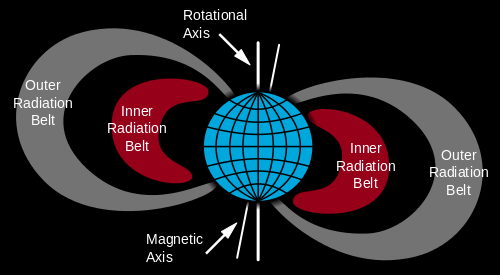
\includegraphics[width=0.5\textwidth]{van_allen_belts.png}
    \caption[Van Allen Radiation Belts]{Cross section of the Van Allen radiation belts.\cite{wikipedia2016vanallen}}
    \label{fig:van_allen_belts}
\end{figure}


\subsection{Directional Radiation Sensor}
\label{sec:radiation_sensor}
A typical radiation sensor is composed of a simple diode (see fig. \ref{fig:detector_diode}).
Reverse biasing of this diode will induce a depletion region in which ionizing particles can be detected.
The passing of such a particle generates charges (electron-hole pairs) in the depletion region, which produce a signal under the action of an electric field.
Since the amount of energy needed to create electron-hole pairs is only dependent on the detector material, the number of created charges can be calculated and therefore the energy of the radiation can be deduced.\cite{rossi2006pixel}

\begin{figure}[H]
    \centering
    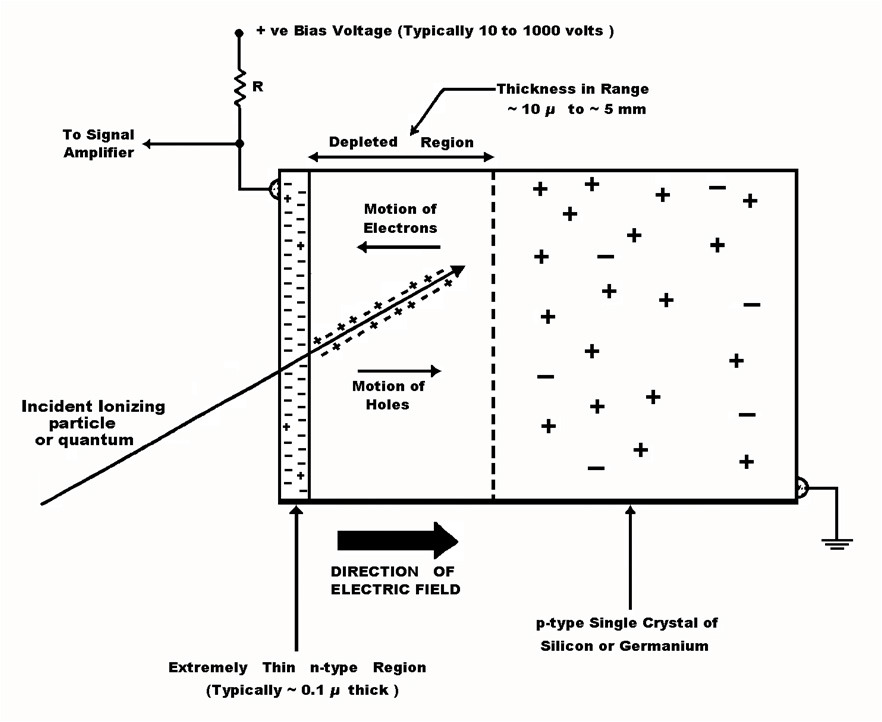
\includegraphics[width=0.5\textwidth]{detector_diode.png}
    \caption[Schematic Detector Diode]{Schematic plot of a single detector diode.\cite{am2016semiconductor}}
    \label{fig:detector_diode}
\end{figure}

The sensor from PSI (see fig. \ref{fig:detector_die}) is a PIPS (Passivated Implanted Planar Silicon) detector.\footnote{The sensor is similar to the one used in the RADEM instrument of the JUICE mission.}
It consists of 31 reverse biased diodes (PN junctions), meaning that their anode should be set to 80V and their cathode to GND.
A copper, dome-shaped stencil (see fig. \ref{fig:detector_stencil}) is used to shield most of the detector from radiation.
Holes in the stencil will enable radiation to fall onto the detector diodes, which are shaped in a way that the wholes project on an equal surface.\footnote{Hence the tear shape of the outer diodes and the round shape of the center diode.}
The whole circular area around the diodes are used as a large anode, it's purpose is to smoothen the electric field lines in the detector junctions and around them.
This is to avoid noise from charges created outside of the detectors and therefore inside the large anode, which are collected and removed using a capacitance.
Guard rings are placed around the large anode, they protect the detectors from leakage current.
The back of the die is connected to a large ground pad, while the detectors, large anode and guard rings are connected via wire-bonding to a PCB.

\begin{figure}[H]
    \centering
    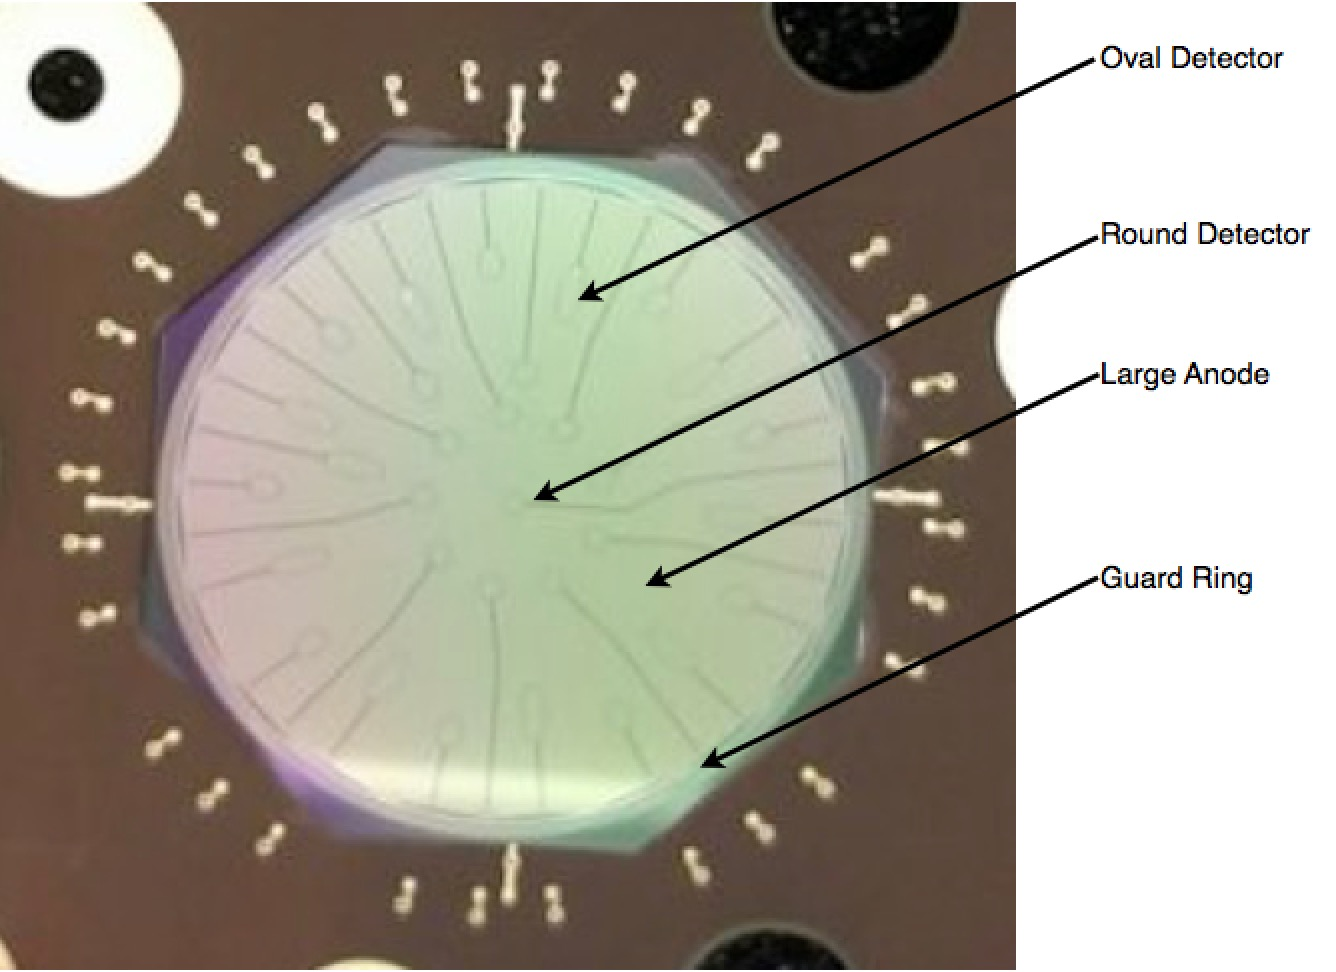
\includegraphics[width=0.5\textwidth]{detector_die.jpg}
    \caption[PSI Detector Die]{Picture of the PSI detector die.}
    \label{fig:detector_die}
\end{figure}

\begin{figure}[H]
    \centering
    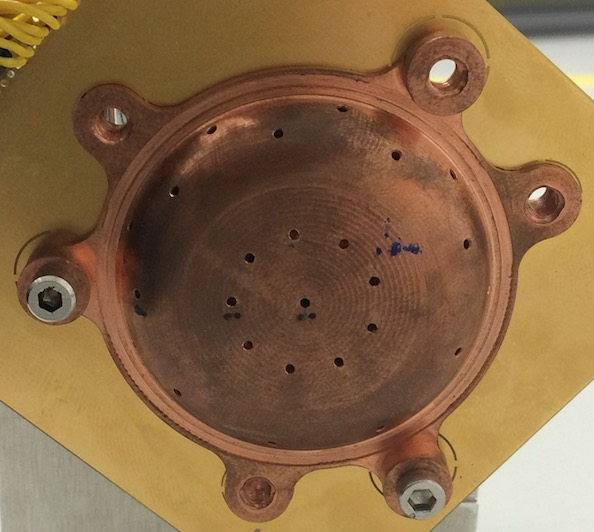
\includegraphics[width=0.5\textwidth]{detector_stencil.jpg}
    \caption[PSI Detector Stencil]{Picture of the PSI detector stencil.}
    \label{fig:detector_stencil}
\end{figure}
 \newpage
\section{Readout Electronic Design}
\label{sec:electronic_design}
The design of the readout electronics depends mainly on the directionality radiation sensor (see sec. \ref{sec:radiation_sensor}) and the ASIC VATA466 (see \cite{Meier2016VATA466}) architecture and drive requirements.
The sensor needs a high voltage supply (see sec. \ref{sec:hv_supply}) to create a reverse bias, the ASIC (see sec. \ref{sec:vata466_baseboard}) is used to readout the sensor data.
The ASIC itself demands some stable supply voltages (see sec. \ref{sec:power_supplies}) and a bias current (see sec. \ref{sec:bias_current}).
To have access to the spectroscopic mode for configuration purposes an ADC (Analog Digital Converter) is needed (see sec. \ref{sec:adc}).
Finally the power and data have to be interfaced with the rest of the cubesat (see sec. \ref{sec:interface_cubesat}).
The block diagram in fig. \ref{fig:electronic_block_diagram} shows the relationship between the different functional blocks of this electronic system.
\begin{figure}[H]
    \centering
    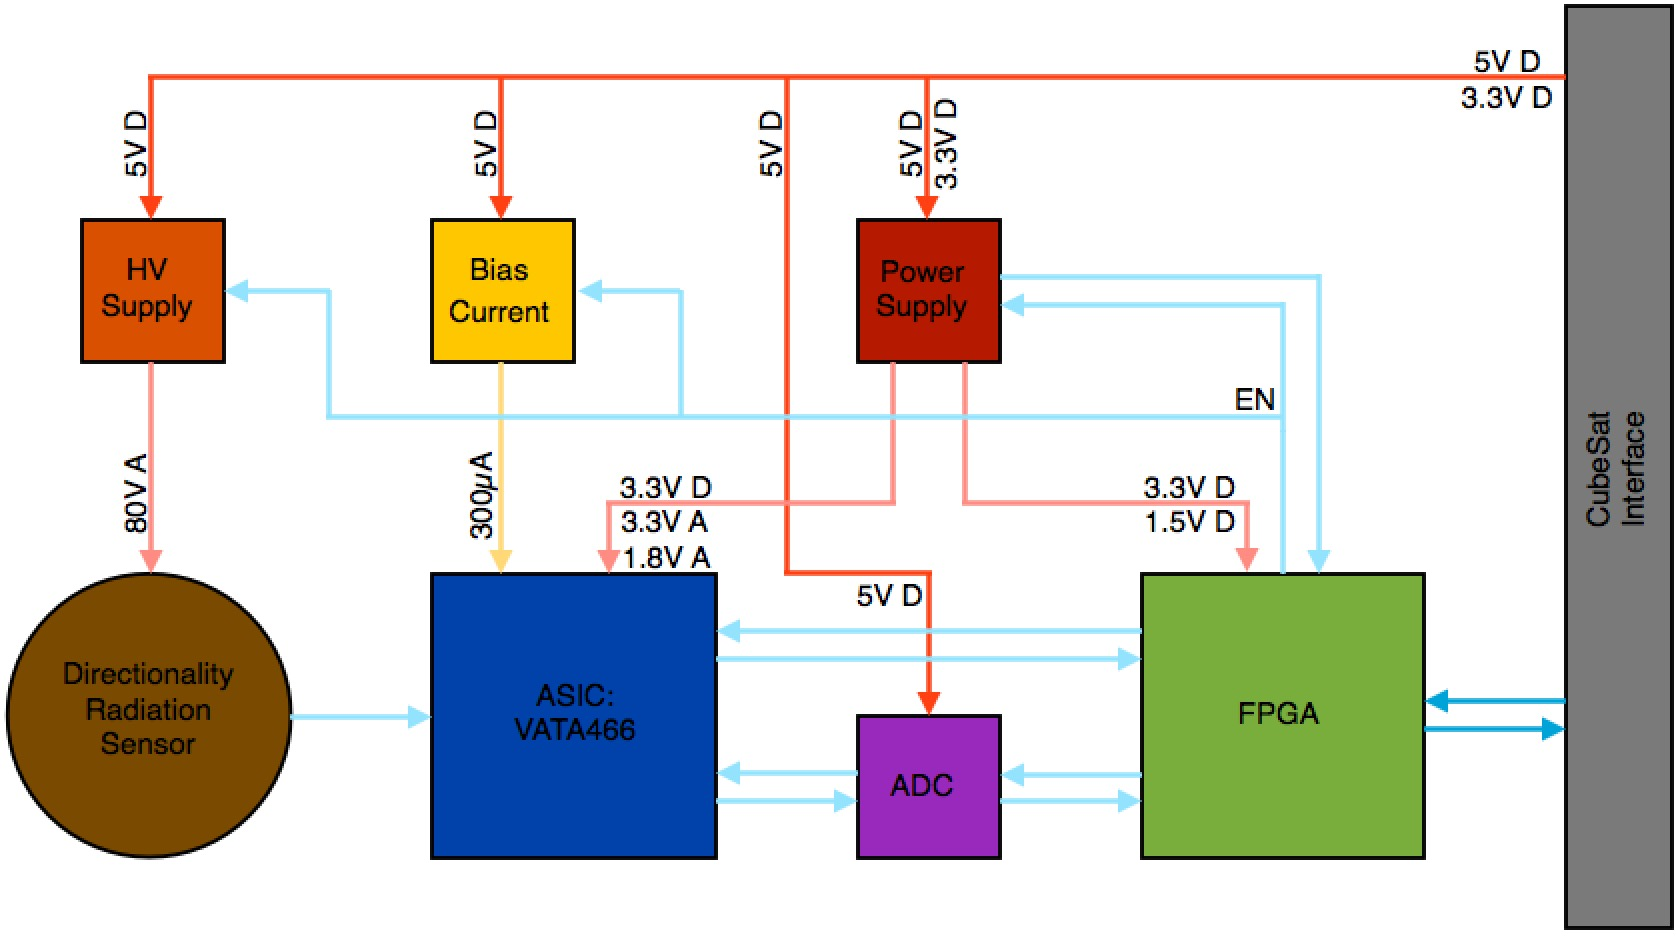
\includegraphics[width=1\textwidth]{electronic_block_diagram.jpg}
    \caption[Block Diagram Readout Electronics]{Block diagram of directional radiation sensor's readout electronics. \\    (Power: Red Arrows; Data: Blue Arrows)}
    \label{fig:electronic_block_diagram}
\end{figure}

The design has to be optimized in terms of power consumption, size and radiation hardness. 
For the latter it was discussed with PSI that the final design could be tested for it's radiation resistance and therefore much cheaper and not officially radiation hardened components can be chosen.
Size and power considerations mainly have to be traded-off against signal quality.
% * <kosheira@gmail.com> 2017-01-13T18:48:56.397Z:
%
% ^.
It is important to stay in the boundaries given by the data sheet of the ASIC to ensure a correct functioning of the instrument.


\subsection{VATA466 Baseboard}
\label{sec:vata466_baseboard}
The schematic ``VATA466\_Base\_Board.SchDoc'' includes all the basic building blocks of the electronic design and therefore resembles largely to the block diagram and description in sec. \ref{sec:electronic_design}.
A data bus connects all the command and data lines between the different modules and the FPGA.
A power bus distributes the correct voltages to the specific systems.

\subsubsection{ASIC: VATA466}
\label{sec:asic}
In the schematic ``VATA466.SchDoc'' the ASIC is divided into his functional subparts.
Figure \ref{fig:signals_pads} shows a schematic representation of the ASIC's functions and pins.
\begin{figure}[H]
    \centering
    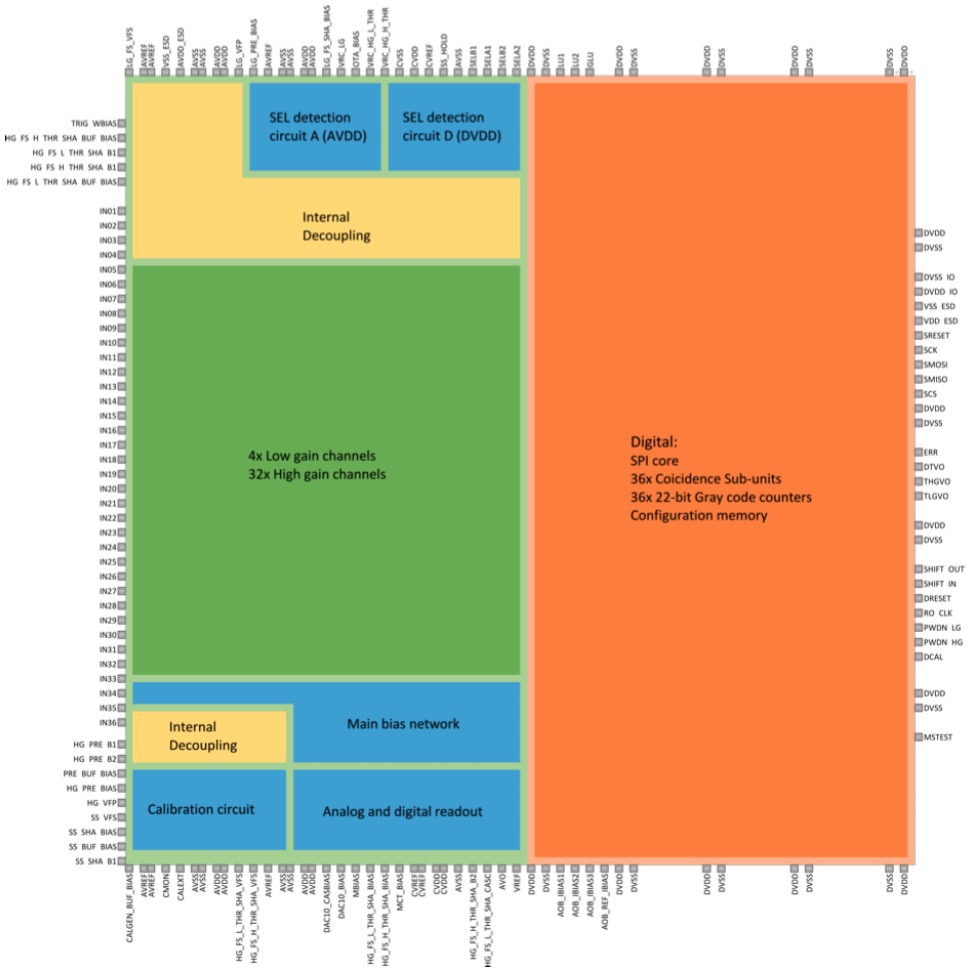
\includegraphics[width=0.7\textwidth]{signals_pads_chip.jpg}
    \caption[Signals and Chip Pad Frame]{Schematic overview of subparts and pins of the ASIC.\cite[p. 14, fig. 3]{Meier2016VATA466}}
    \label{fig:signals_pads}
\end{figure}

There are 36 CSA (charge sensitive pre-amplifiers), called U19A in the schematics, 4 of them have a low gain and 32 a high gain.
The DRS has 31 detector diodes and therefore uses 31 inputs of the high gain channels.

The ASIC also contains two power subparts, an analogue one (U19B) and a digital one (U19C).
They differ in that the analogue input voltages have strict requirements and need to have low noise since they are going to interact directly with the signals in the ASIC.
The digital input voltage is only used for the logic in the ASIC and is therefore less critical.
These inputs should be strictly isolated to avoid any degradation of the measurements.
The supply voltages will be discussed in more detail in section \ref{sec:power_supplies}.

The next subunit of the ASIC holds all his bias and test-pads (U19D).
The bias network will be described in more detail in section \ref{sec:bias_current}.
The test-pads can be used to debug the ASIC and to directly readout some of it's internal signals.
The following table describes the pins purposes and gives recommendations for external decoupling:
\begin{table}[h!]
	\centering
    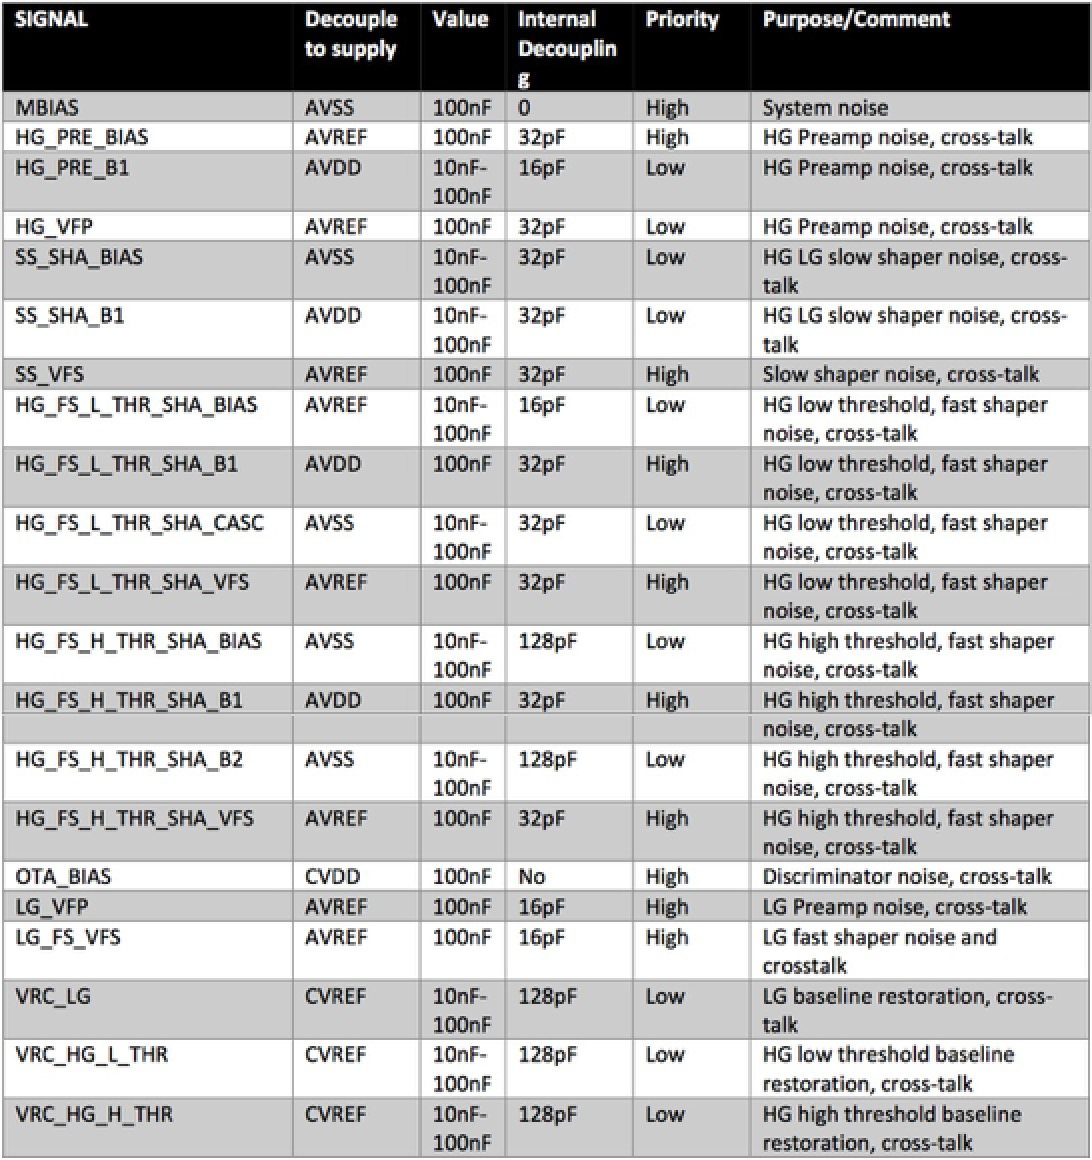
\includegraphics[width=0.7\textwidth]{test-pins.jpg}
    \caption[Test-pins Purpose and External Decoupling]{Purposes of the different test-pins and recoomendations for external decoupling.\cite[p. 65, tab. 31]{Meier2016VATA466}}
	\label{tab:test-pads}
\end{table}

The last subpart of the ASIC regroups all pins used for the readout and commands (U19E).
It uses SPI (Serial Peripheral Interface) to read or write over the ASIC's registers and thereby enables the use of the counting mode.
A calibration subunit can be used to test and calibrate the gain in the pre-amplifier, slow shapers and trigger the increment of a counter in a channel.
The power down block is used to power down the 4 low gain channels (1 to 4) and\/or 16 high gain channels (21 to 36), channels 5 to 20 are always powered on.
A single analogue output is provided through the AVO pin, which allows the readout of the pulse heights from all channels via multiplexing (see sec. \ref{sec:adc}).
The multiplexer is controlled through the A\&D channel readout block and is therefore used to setup the spectroscopic mode of the ASIC.
The trigger out block is used to indicate the triggering of either a low-gain or high-gain channel or the digital multiplexer.
The last block enables the latch-up detection in the ASIC and will be further explained in the next section.\cite{Meier2016VATA466}

\subsubsection{Latch-up Detector}
\label{sec:latchup_detector}
There are two latch-up detection modules included in the ASIC.
They each have two inputs SELA and SELB and one output LU.
A global latch-up signal (GLU) is created through a logic OR between the two latch-up detector outputs.
The schematic ``Latch\_Up\_Power.SchDoc'' represents an implementation of the recommended external circuit (see fig. \ref{fig:latch-up}).
\begin{figure}[H]
    \centering
    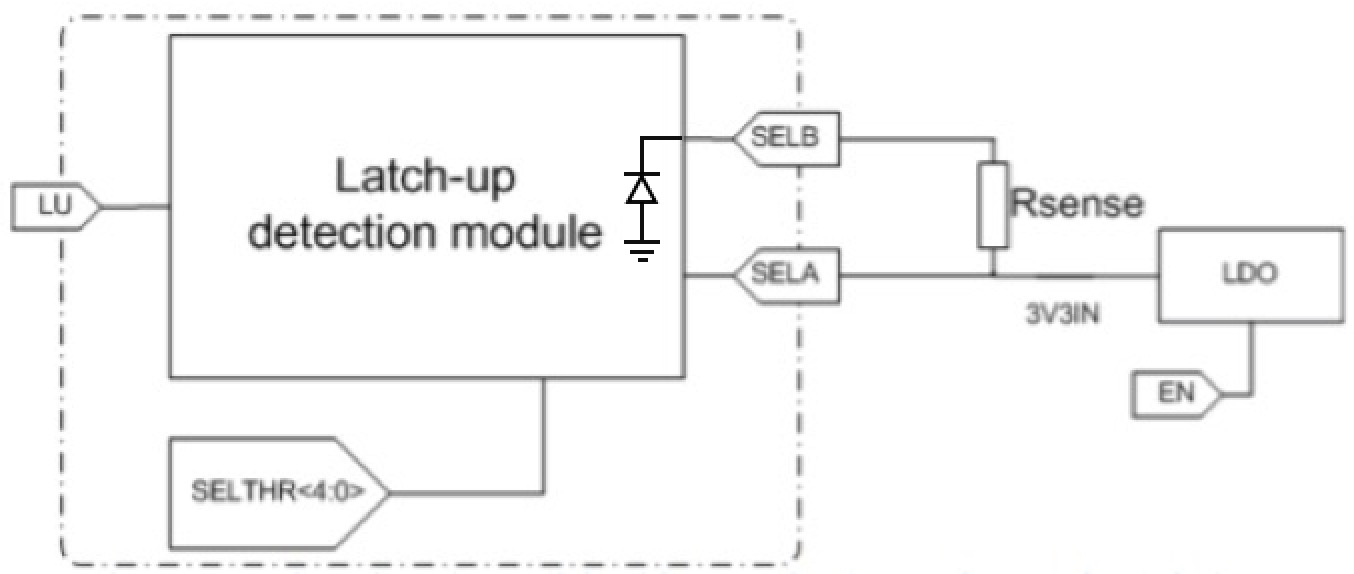
\includegraphics[width=0.6\textwidth]{latch-up.jpg}
    \caption[Latch-up Detection Module]{Reference design of an external latch-up detection circuit.\cite[p. 66, fig. 12]{Meier2016VATA466}}
    \label{fig:latch-up}
\end{figure}

The circuit consists of a LDO (U7 \& U8\footnote{LT1763}) which provide a constant 3.3V.
The detector can be seen as a simple diode.
As long as there is no SEL (Single-Event Latch-up), there will be no voltage drop over $R_{sense}$.
A SEL would make the diode conducting and there would be a voltage drop between the SELA and SELB pins.
This voltage is compared to the threshold value (SELTHR).
Being above it, the corresponding LU pin is set to high and therefore the GLU pin will go to high as well and indicate a latch-up detection.\cite[p. 66-68, fig. 12]{Meier2016VATA466}


\subsection{High Voltage Supply}
\label{sec:hv_supply}
A high voltage supply is needed to induce the reverse bias on the DRS's diodes.
Depending of their lifetime and sensitivity they should be biased with about 40-60 V.\footnote{A bias of 80V could be imagined, which might make it possible to share a single high voltage supply between the DRS from PSI and the sensors from RUAG.} 

The circuit ``HV\_Power.SchDoc'' uses an extra-small high voltage biasing supply (U9\footnote{0.1XS5-P0.1}.
A 5V input voltage is required to create a 0-100V output voltage with a maximum output current of 1mA.
To adjust the high voltage output, an 12 bit DAC (Digital Analog Converter) with reset to zero scale (U10\footnote{LTC2631}) was chosen, which produces .
The zero scale reset is important to prevent uncontrolled voltage spikes on power-on and therefore make the system initialization consistent and repeatable.
The DAC produces an output voltage of 0-2.5V which is proportional to the high voltage output of the supply of 0-100V.
A serial $I^2C$ interface is used to operate the DAC.


\subsection{Directionality Sensor}
\label{sec:directionality Sensor}
As explained in section \ref{sec:radiation_sensor}, the DRS is composed of 31 sensing diodes, a large anode and guard rings.

In the ``Sensor\_Diodes.SchDoc'' schematic a typical connection of the sensing diodes is shown.
A high voltage (40-80V) is applied on the cathode and the anode is connected to GND to apply the reverse bias.
When radiation passes through the depletion region a current is induced.
This current passes through a resistor, so that at the output a voltage can be read.
The trade-off for this resistor is done between the resistivity and noise, a value of $2.2M\Omega$ was defined by PSI.

The schematic ``Shield\_Sensor.SchDoc'' shows both, the concept of the large anode and a guard ring.
Both are split up in 4 equal sub-circuits.
This approach allows a symmetric distribution of the contacts around the circular detector, which in turn makes the protective effects more symmetric and therefore more effective. 

The large anode is basically connected with a resistor and capacitor.
The resistor will define current flow and the capacitor will collect the created charges to avoid noise from the area around the detector diodes.
The capacitors should be chosen as big as possible, so that a large number of charges can be buffered.
On the other hand this capacitor needs to be compatible with the large biasing voltage, which implies a larger footprint.
A trade-off has to be done considering the footprint of the capacitor.

The guard rings are rings of reverse biased diodes.
They will define the outer edge of the depletion region of the large anode and the sensors.
This is implemented to avoid leakage currents from the outside of the detector.


\subsection{Supply Voltages}
\label{sec:power_supplies}
- trade-off housekeeping

\subsubsection{Analog Supply Voltages}
\label{sec:analog_supply}
- 1.8 V, 3.3 V
- digital vs opto copplers

\subsection{Bias Current}
\label{sec:bias_current}


\subsection{Analog Digital Converter}
\label{sec:adc}


\subsection{Interface CubeSat}
\label{sec:interface_cubesat}
 \newpage
\section{Digital Communication Interface and Readout}
\label{sec:logic_design}


\subsection{Description of the ASIC digital subsystem}
\label{sec:descriptionASIC}


\begin{figure}[H]
    \centering
    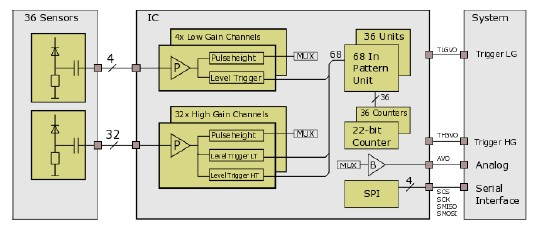
\includegraphics[width=1\textwidth]{ASIC_schematic.jpg}
    \caption[]{Block Diagram Schematic of the ASIC (VATA466/ide3466) (\cite{Meier2016VATA466}) }
    \label{fig:ASIC_schematic}
\end{figure}

\subsubsection{Input Channels}

From the figure above it can be seen that each diode anode is AC-coupled to one input. The ASIC has 4 Low Gain (LG) channels and 32 High Gain (HG) channels, which serve as input from the detector diodes of the directionality sensor. Each channel has one pre-amplifier and an analogue processing for pulse height and level triggers. In the figure below, the channel inputs are depicted on the left side of the scheme.

\begin{figure}[H]
    \centering
    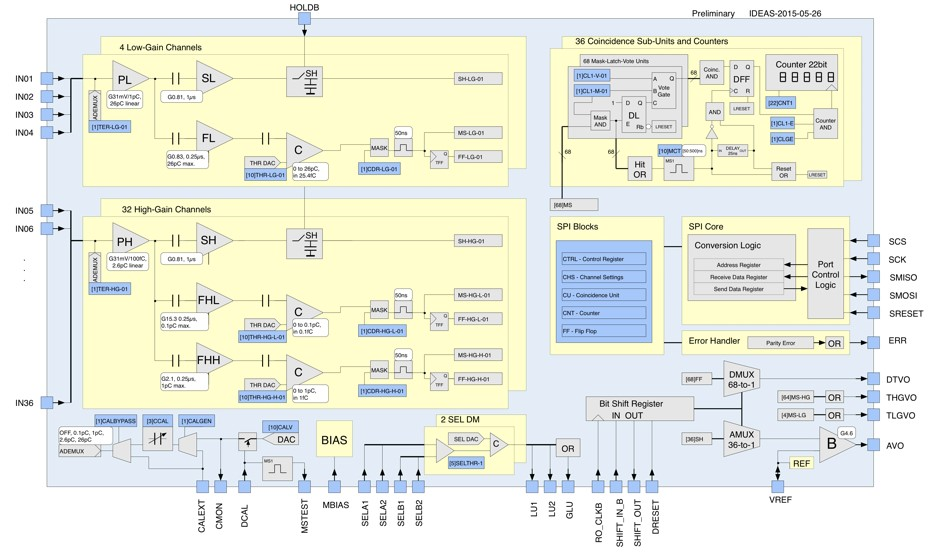
\includegraphics[width=0.9\textwidth]{ASIC_Functional.jpg}
    \caption[]{ASIC functional schematic with I/O (VATA466/ide3466) (\cite{Meier2016VATA466}) }
    \label{fig:ASIC_Functional}
\end{figure}

\subsubsection{Modes of operation}

The ASIC has two modes of operation and each of the modes requires a different approach for the readout. It can be used in the Counting Mode Acquisition (CMA) or Spectroscopic Mode Acquisition (SMA). 
\newline
The CMA is the mode for which the digital hardware was designed. In this mode, the values of a total of 36 registers, which comprise the so-called Coincidence Sub-Unit (CSU) of the ASIC, can be read. The CMU, its registers and configuration principle is described later in this section. The value in each of the registers reflects the number of events that occurred, which fulfill the requirements of any individual out of 36 prior defined coincidences.
\newline
The following steps are required to run this mode successfully:





\begin{itemize}
\item Configuration of the analogue channel thresholds through channel configuration registers

\item Configuration of the coincidence units with channel trigger coincidence and anti-coincidence through Coincidence Sub-Unit configuration registers
\item Periodic read-out of the coincidence counter registers

\end{itemize}

The SMA mode will only be explained briefly in this report.
Its objective is to recreate the shape of the detected
pulses. The pulses which are registered in the input
channels can be transformed to 36 analogue values by a slow
shaper and can be later read out serially with the help of
an analogue multiplexer (36-to-1 AMUX) that is controlled
by the RO\_CLKB, SHIFT\_IN\_B and DRESET inputs as seen in
\ref{fig:ASIC_Functional}, the signal SHIFT\_OUT
indicates when the operation is finished.

The parts of the subsystem will be described with regards to the counting mode acquisition. 

\subsubsection{Registers}

The registers in the ASIC have a length of 22 bit, each register can be mapped to by a 9-bit address.

\subsubsection{Channel Thresholds}

Each of the low gain channels has one and each of the high gain channels has two channel configuration registers associated with them. The values in the registers determine the charge threshold for their respective comparator. In the ASIC, a digital pulse is generated when the amount of charge that is generated at the respective input channel exceeds the value defined in the comparator. One threshold can be set for the low gain channels and two thresholds can be set for the high-gain channels, hence the need for 2 channel configuration registers for the HG channels.

\subsubsection{Coincidence Unit}

There are in total 36 CSUs. Each sub-unit is associated with 7 CSU configuration registers, that collectively define a coincidence. A coincidence is essentially a combination of digital pulses that were triggered based on the set channel thresholds. In the configuration registers, it can be defined if a channel shall be considered in a coincidence through a mask bit and whether it must have triggered through a coincidence / anti-coincidence (C/Ac) bit. If the triggered digital pulses fulfill the coincidence requirements, the specific CSU’s counter is increased by one. The reason we need 7 configuration registers for each CSU is the following: 
\newline
There are four LG channels, each with one (C/Ac) bit and one mask bit. And 32 HG channels, each with two thresholds and each of the thresholds with one (C/Ac) bit and one mask bit).

\begin{equation}
\lceil{\frac{\left(4\cdot2 + 32 \cdot 2 \cdot 2 \right)}{22\cdot bits/register}}\rceil = \lceil{6.18}\rceil \hphantom{\cdot}  registers = 7 \hphantom{\cdot} registers
\end{equation}

The values of the Coincidence Sub-Unit counters cannot be reset, this is for the sake of increasing the radiation tolerance of the design.

\subsubsection{Communication Interface}

The configuration registers can be read or written via the digital SPI port of the ASIC. The registers which contain the current values of the coincidence counters can only be read and not written through SPI. The communication constitutes a single Master to Single slave interface, whereas the ASIC takes the role of the Slave and the user logic in the digital design implements the corresponding Master.

\begin{figure}[H]
    \centering
    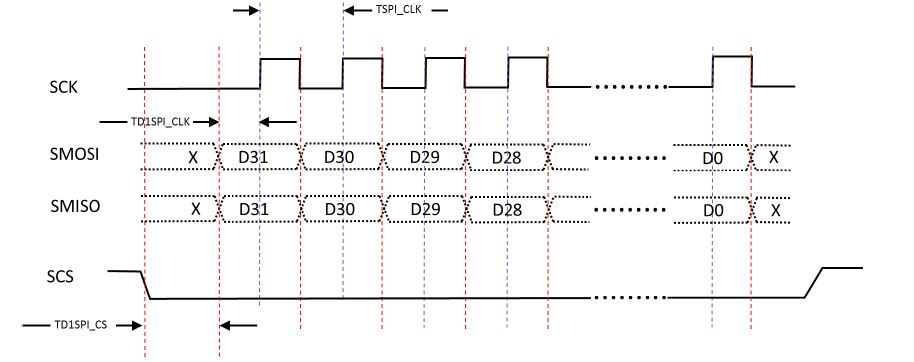
\includegraphics[width=0.9\textwidth]{SPI_Timing.jpg}
    \caption[]{SPI-Timing diagram) }
    \label{fig:SPI_Timing}
\end{figure}

The following definitions hold for the ASIC in use:


\begin{table}[H]

\caption[]{SPI Definitions}
    \label{tab:1}
    
  \begin{center}  
  \begin{tabular}{|r|l|}
  \hline
  \textbf{Name}  & \textbf{Definition} \\ \cline{1-2}
  
  \textbf{SCK} & SPI Serial Clock (output from Master) \\
  \textbf{SMOSI} &Master Output, Slave Input \\ 
  \textbf{SMISO} &Master Input, Slave Output\\
  \textbf{SCS} &Chip-Select (Active low, provided by Master)\\
  \hline
  
\end{tabular}
\end{center}
\end{table}


During one SPI communication cycle, the 32-bit word in the following configuration is sent to the ASIC serially on the SMOSI line.

\begin{table}[H]

\caption[]{Master to Slave serial bit-fields}
    \label{tab:2}
    
  \begin{center}  
  \begin{tabular}{|l|c|c|c|}
  \hline
  \textbf{Bit indices}  & 31 to 23  & 22 & 21 to 0\\ 
  \hline
  \textbf{Data Components} & SPI-Address & Read/Write Bit & SPI-Data \\
  \hline
  
\end{tabular}
\end{center}
\end{table}

The 32-bit word in the following configuration is sent from the ASIC serially on the SMISO line.

\begin{table}[H]

\caption[]{Slave to Master serial bit-fields}
    \label{tab:3}
    
  \begin{center}  
  \begin{tabular}{|l|c|c|c|}
  \hline
  \textbf{Bit indices}  & 31 to 23  & 22 & 21 to 0\\ 
  \hline
  \textbf{Data Components} & Meaningless & Meaningless & SPI-Data \\
  \hline
  
\end{tabular}
\end{center}
\end{table}
The SPI serial clock operates at minimum frequency of 1 kHz and at a maximum frequency of 5 MHz

\subsection{Design of digital hardware}
\label{sec:hardwaredesign}
\subsubsection{Introduction}

The language chosen for hardware generation is VHDL. The code was written and tested in the Libero SoC v11.7 integrated development environment. The company, which developed the environment is called Microsemi. They also provide pre-defined soft-cores such as the Core\_Uart which is used in the design. The hardware consists of a processing unit which takes commands from a computer, in the case of the CubeSat mission, this would be the on-board computer. The processing unit deciphers the input commands and interacts with the on-fabric memory as well as the ASIC. The testbenches are written in VHDL as well and the simulation software is called ModelSim and is automatically called from the Libero Interface and performs the simulation based on the specification in the testbench file. Many of the hardware components already existed in an undocumented form for the ASIC test board at PSI. The code for these components was written by Carla Brito from the company Efacec.


\subsubsection{Functional Block Diagram}

\begin{figure}[H]
    \centering
    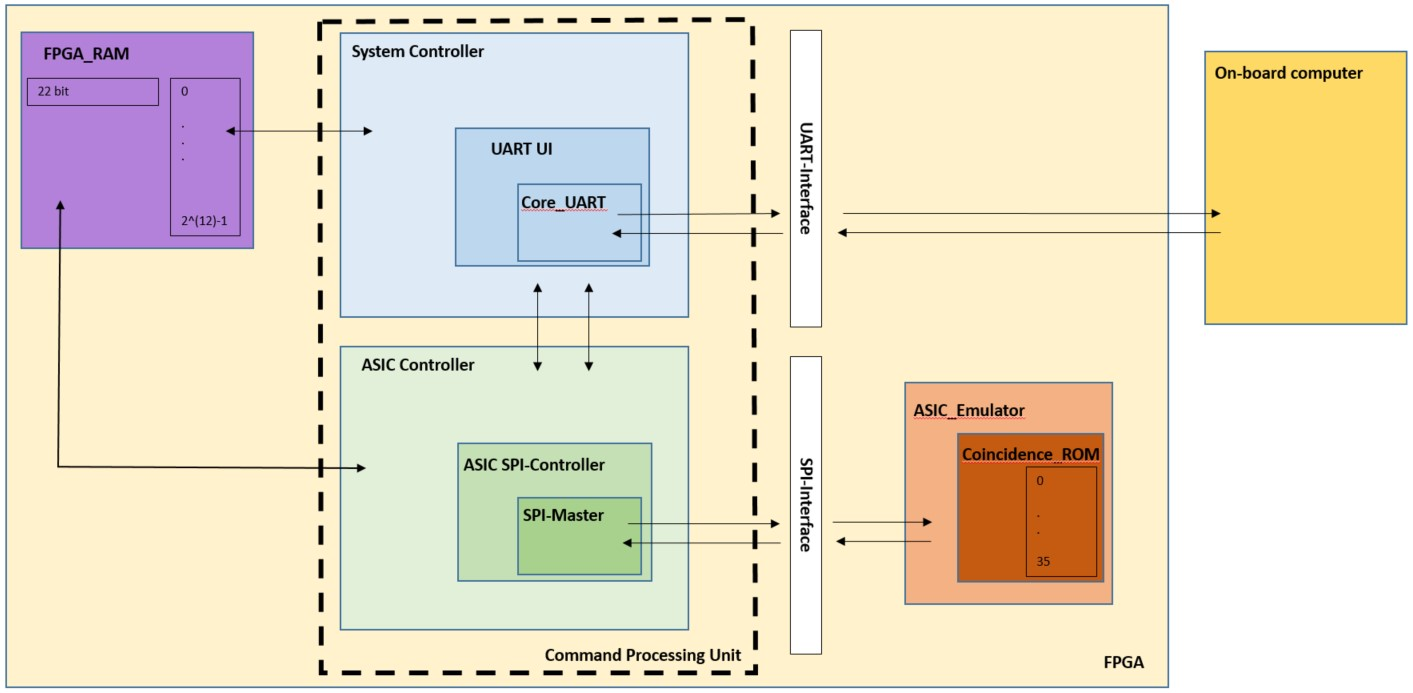
\includegraphics[width=0.9\textwidth]{Fucional_block.jpg}
    \caption[]{Functional block diagram implemented with VHDL logic) }
    \label{fig:Functional_block}
\end{figure}

The diagram above shall visualize the data flow on the FPGA architecture.

The diagram does not consider the connections and lines for the clock. In the Microsemi Libero environment, an on-board clock can be generated by connecting the output of the chip oscillator with a clock conditioning circuit, which generates the desired frequencies.
\newline

The memory on the FGPA is implemented using a RAM component. It stores data which is organized in the 22-bit format following the register size of the ASIC. It consists of 4096 readable and writeable addresses and therefore constitutes a memory of about 90 Kbit. The functionality and properties of the other blocks will be explained in their separate section later.
\newline

The oscillator in conjunction with the clock conditioning circuit generates a clock, which runs at a frequency of 20 MHz and is used for all the components except the ASIC emulator, who depends on the SPI-clock, which runs at a rate of 200 kHz.

\subsubsection{Bit-field logic of commands}
The half-duplex mode communication between the computer and the FPGA works via a serial UART interface utilizing 40-bit words.
\newline

Generally, the computer-to-FPGA commands have the following bit-field logic:

\begin{table}[H]

\caption[]{Computer-to-FPGA command constellation}
    \label{tab:4}
    
  \begin{center}  
  \begin{tabular}{|c|p{2cm}|p{2cm}|p{2.5cm}|p{2cm}|p{2cm}|}
  \hline
  \textbf{Bit indices forward}  & 39 to 36  & 35 & 34 & 33 to 22 & 21 to 0\\ 
  \hline
  \textbf{Data Components} & Command \newline Type & NO USE & Local Usage & Command Control Address & Data bits \\
  \hline
  
\end{tabular}
\end{center}
\end{table}

The FPGA-to-computer responses are in the following configuration:


\begin{table}[H]

\caption[]{FPGA-to-computer response constellation}
    \label{tab:5}
    
  \begin{center}  
  \begin{tabular}{|c|p{3cm}|p{3cm}|p{3cm}|}
  \hline
  \textbf{Bit indices response}  & 39 to 36  & 35 to 22 & 21 to 0 \\ 
  \hline
  \textbf{Data Components} & Command Type Response & Copy of computer-to-FPGA indices for verification & Data from memory or ASIC register data or copy of computer-to-FPGA indices for verification \\
  \hline
  
\end{tabular}
\end{center}
\end{table}

To write data to an ASIC register via the SPI-port, the following sequences must be sent via the UART port:


\begin{table}[H]

\caption[]{Write ASIC register command 1/2}
    \label{tab:6}
    
  \begin{center}  
  \begin{tabular}{|c|p{2cm}|p{2cm}|p{2.5cm}|p{2cm}|p{2cm}|}
  \hline
  \textbf{Bit indices}  & 39 to 36  & 35 & 34 & 33 to 22 & 21 to 0\\ 
  \hline
  \textbf{Values} & 0001  & 0 & 0 & 0x00A & Data bits \\
  \hline
  
\end{tabular}
\end{center}
\end{table}

\begin{table}[H]

\caption[]{Write ASIC register command 2/2}
    \label{tab:7}
    
  \begin{center}  
  \begin{tabular}{|c|p{1.5cm}|p{0.7cm}|p{1cm}|p{1cm}|p{1cm}|p{2cm}|p{2cm}|}
  \hline
  \textbf{Bit indices}  & 39 to 36  & 35 & 34 & 33 to 22 & 21 to 10 & 9 & 8 to 0\\ 
  \hline
  \textbf{Values} & 0001  & 0 & 0 & 0x009 & Meaningless, set to 0 & R/W bit, set to 1 & SPI register address \\
  \hline
  
\end{tabular}
\end{center}
\end{table}

To read data from an ASIC register via the SPI-port, the following sequences must be sent via the UART port:

\begin{table}[H]

\caption[]{Read ASIC register command 1/2}
    \label{tab:8}
    
  \begin{center}  
  \begin{tabular}{|c|p{1.5cm}|p{0.7cm}|p{1cm}|p{1cm}|p{1cm}|p{2cm}|p{2cm}|}
  \hline
  \textbf{Bit indices}  & 39 to 36  & 35 & 34 & 33 to 22 & 21 to 10 & 9 & 8 to 0\\ 
  \hline
  \textbf{Values} & 0001  & 0 & 0 & 0x009 & Meaningless, set to 0 & R/W bit, set to 0 & SPI register address \\
  \hline
  
\end{tabular}
\end{center}
\end{table}

\begin{table}[H]

\caption[]{Read ASIC register command 2/2}
    \label{tab:8}
    
  \begin{center}  
  \begin{tabular}{|c|p{1.5cm}|p{0.7cm}|p{1cm}|p{1cm}|p{3cm}|}
  \hline
  \textbf{Bit indices}  & 39 to 36  & 35 & 34 & 33 to 22 & 21 to 0 \\ 
  \hline
  \textbf{Values} & 0000  & 0 & 0 & 0x00D & Meaningless, set to 0  \\
  \hline
  
\end{tabular}
\end{center}
\end{table}

\subsection{System Description}
In this chapter, the individual blocks of the VHDL design are documented in detail.

\subsubsection{UART UI (User Interface)}
This component is responsible for several tasks. First, it converts the serial one line UART RX input into a parallel data line. At the same time, it is responsible for sending a desired output given as parallel register content via the serial UART TX port. For this reason, the sub-block Core UART is employed in this component. It is a native soft core, which means that it is synthesizable pre-written hardware that can be instantiated several times. This softcore is available on the SmartFusion2 as well as the ProASIC3 FPGAs. The core can receive one byte at a time via the serial UART RX port in the following fashion:

\begin{figure}[H]
    \centering
    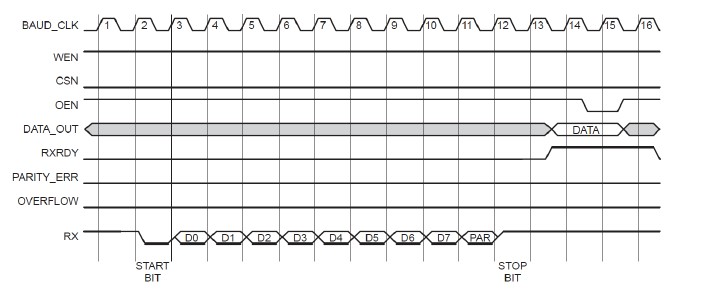
\includegraphics[width=0.89\textwidth]{UART_serial_rx.jpg}
    \caption[]{UART serial receive (\cite{UART}) }
    \label{fig:UART_serial_rx}
\end{figure}

Likewise, one byte at a time can be sent by putting the data at the DATA\_IN port of the Core and setting the WEN (write enable) to active low for at least one clock cycle

\begin{figure}[H]
    \centering
    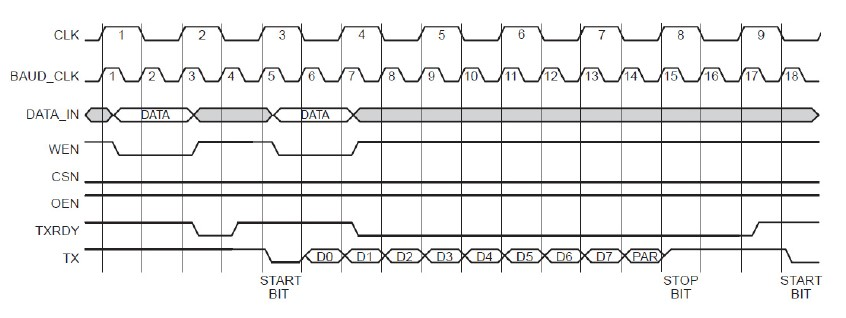
\includegraphics[width=0.89\textwidth]{UART_serial_TX.jpg}
    \caption[]{UART serial transmit (\cite{UART}) }
    \label{fig:UART_serial_TX}
\end{figure}
The Core is operating with the following UART parameters:


\begin{table}[H]

\caption[]{UART Core specifications}
    \label{tab:9}
    
  \begin{center}  
  \begin{tabular}{|r|l|}
  \hline
  \textbf{Parameter}  & \textbf{Value} \\ \cline{1-2}
  
  \textbf{Clock rate} & 20 MHz \\
  \textbf{Baud Rate [Hz]} & 460800\\ 
  \textbf{Baud Rate Adjust} & +0.712 \\
  \textbf{Bit Width} & 8\\
  \textbf{Active Chip Select} & Low \\
  \textbf{Enable Parity} & Yes \\
  \textbf{Parity Type} & Odd \\
  \hline
  
\end{tabular}
\end{center}
\end{table}


However, this is not everything that has to be done, since one command consists of 40 bits a total of 5 bytes need to be sent through the UART port. The UART UI therefore needs to keep track of how many bytes have already been received and re-construct the 40 bit-word by assembling 5 bytes together. Afterwards, the command data and command address must be separated and stored in their designated data lines to be processed by the System Controller, which is one hierarchy stage above the UART UI.

\begin{figure}[H]
    \centering
    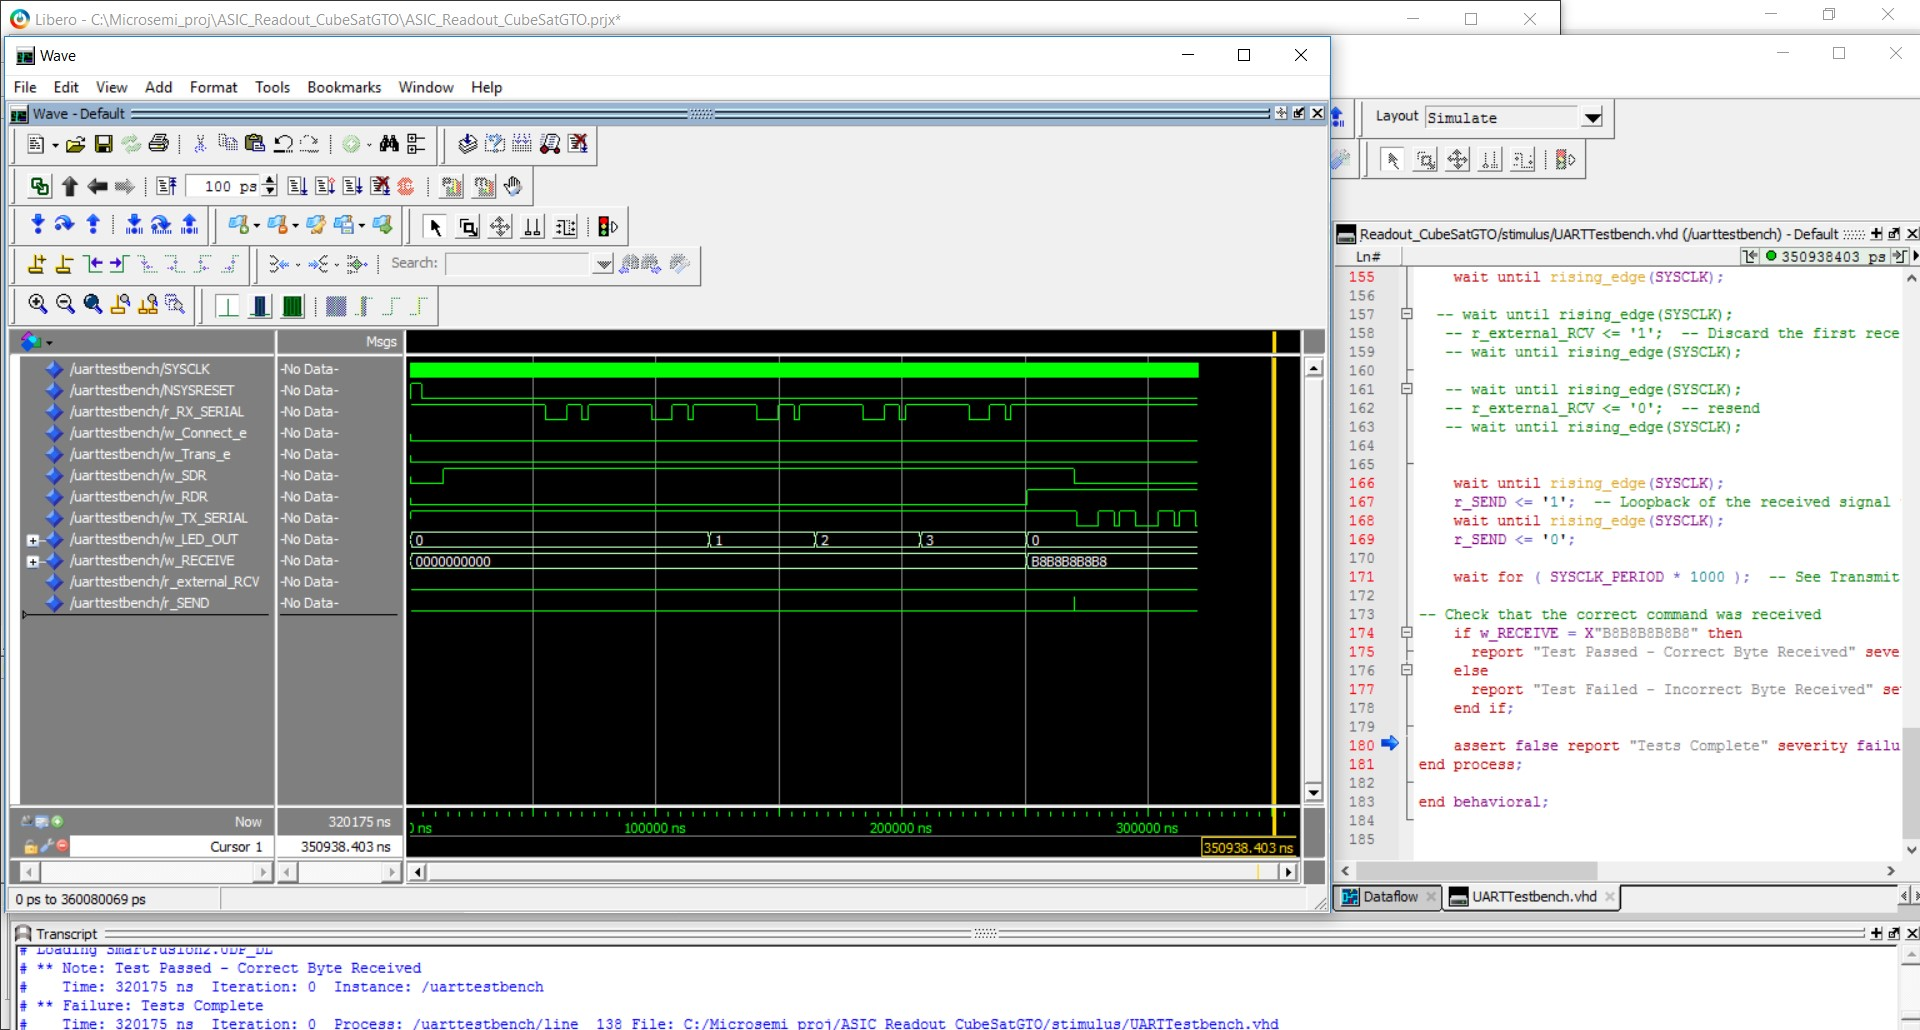
\includegraphics[width=0.89\textwidth]{UART_SIMULATE.jpg}
    \caption[]{UART Interface Test Bench and Simulation) }
    \label{fig:UART_SIMULATE}
\end{figure}

In the wave diagram above, the r\_RX\_SERIAL port depicts the UART input, that is instructed to serially send data to be received by the UART UI. The 40-bit word is successfully re-constructed and stored in the w\_RECEIVE register and via the r\_SEND signal, the serial UART transmit operation can be initiated and the result can be observed on the w\_TX\_SERIAL data line.
\subsubsection{System Controller}
The system controller is the main part of the command processing unit. It deciphers the instructions and controls the data flow accordingly. If instructed to read or write ASIC registers, it is responsible for the delivering of the command data as well as the command address to the ASIC Controller, which is the component that initiates the communication with the ASIC. Furthermore, after each successfully received instruction, the system controller builds the appropriate response and sends it automatically back to the computer via the serial UART transmit port. If instructed to read memory, one command is enough to either read or write a memory address specified in the command address portion of the instruction and immediately send back the data in the memory address to the computer. Due to its relative complexity, a diagram of its state machine has been created.

\begin{figure}[H]
    \centering
    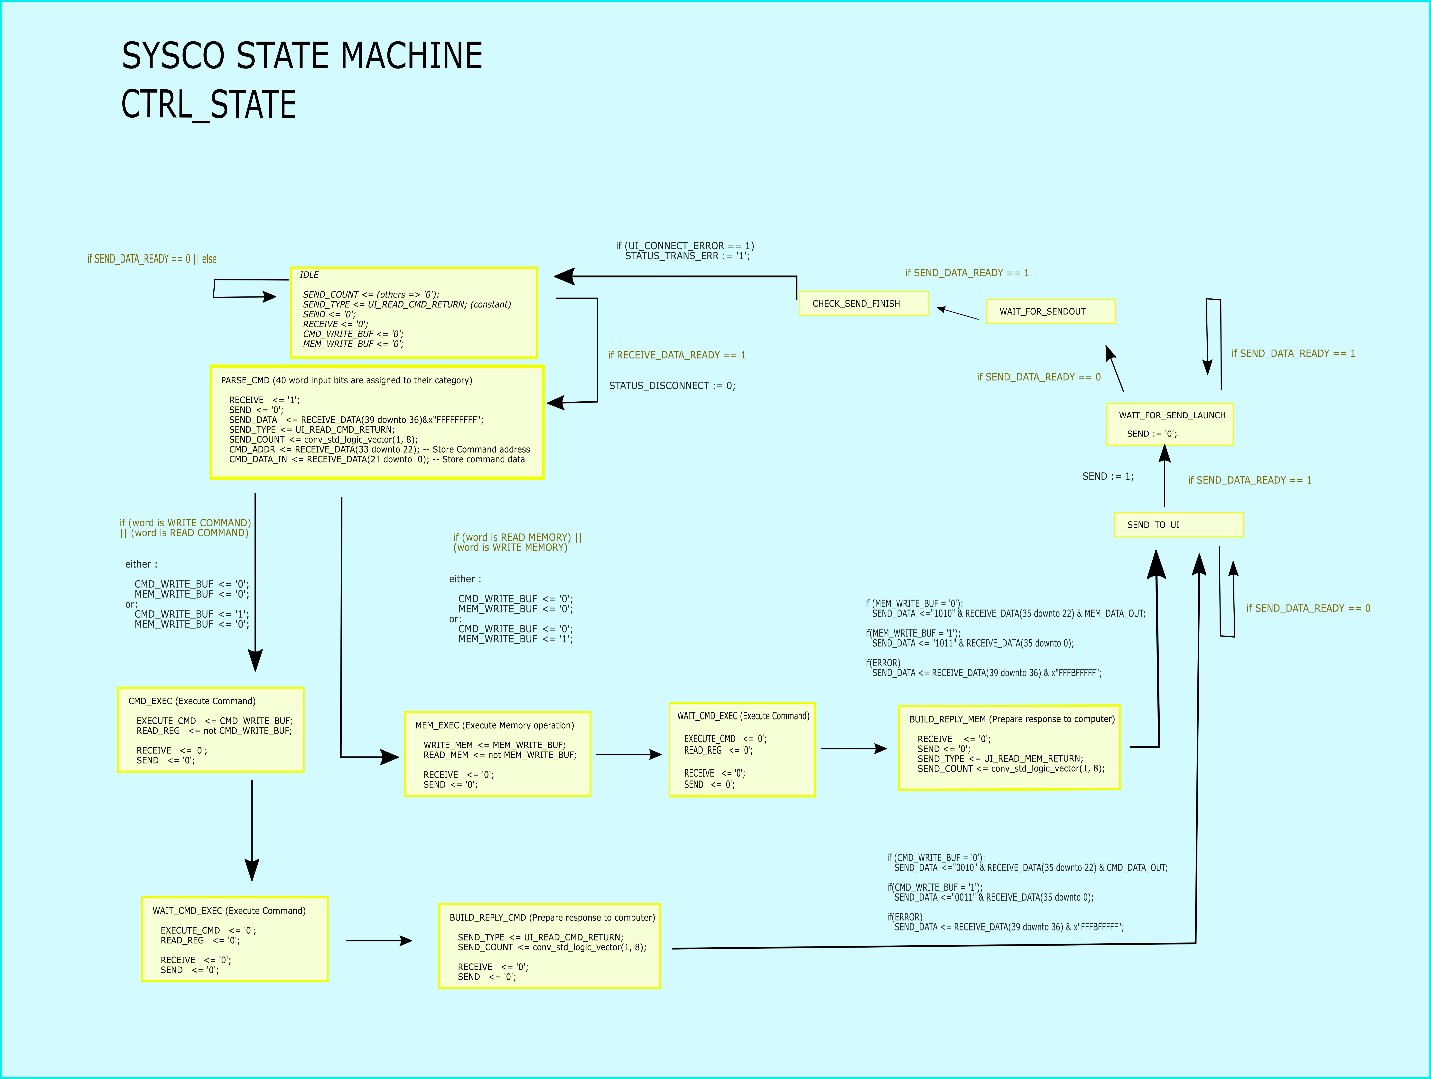
\includegraphics[width=0.89\textwidth]{SYSCO_StateMachine.jpg}
    \caption[]{State machine of the system controller) }
    \label{fig:SYSCO}
\end{figure}
Another testbench has been written to simulate the System Controller design.

\begin{figure}[H]
    \centering
    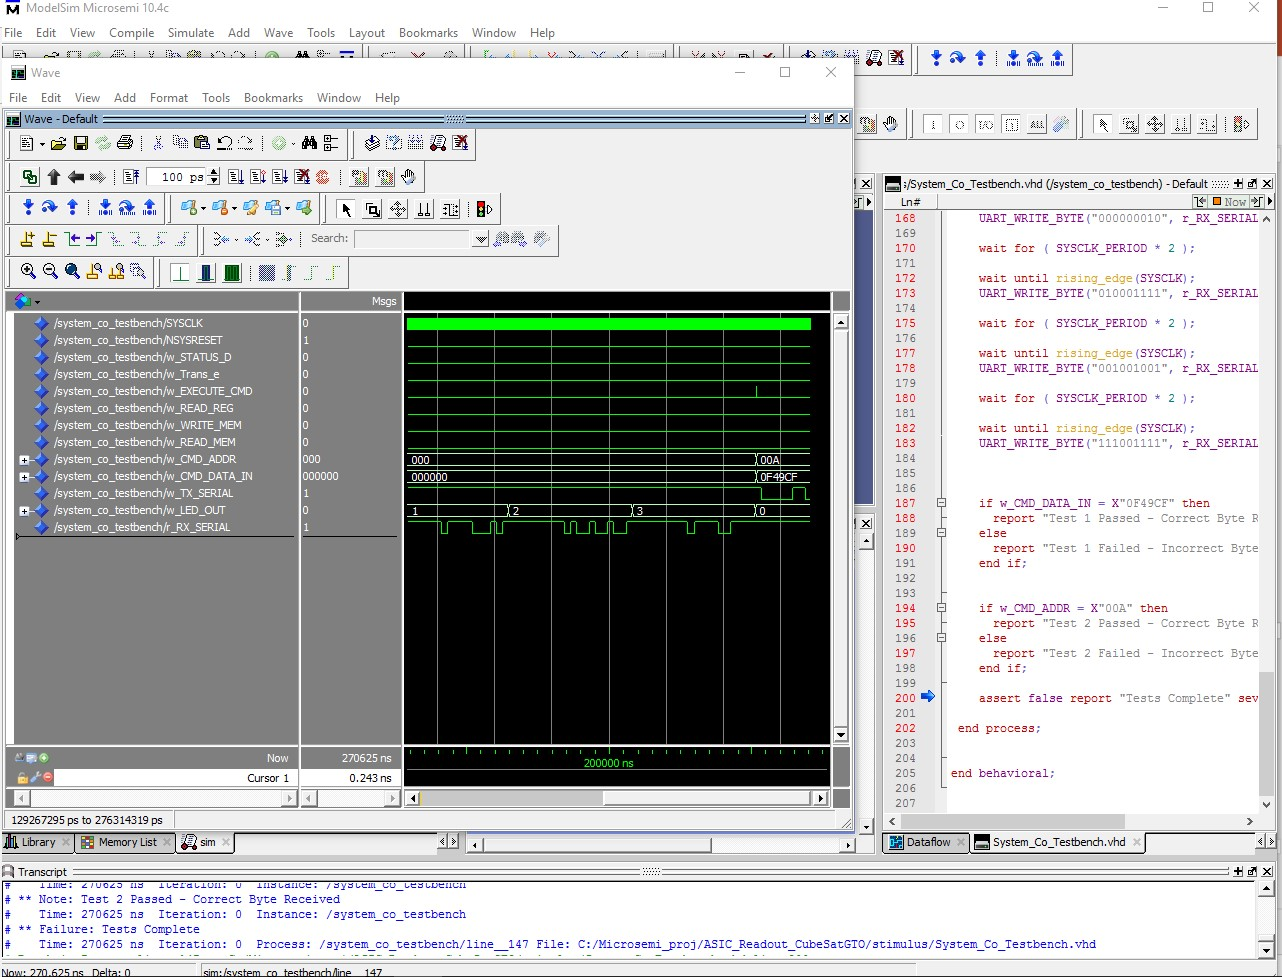
\includegraphics[width=0.8\textwidth]{SYSCO_Simulate.jpg}
    \caption[]{Simulation of the System Controller }
    \label{fig:SYSCO_Sim}
\end{figure}

In this example, like the one described for the UART UI, an instruction is sent through the r\_RX\_SERIAL port, the System Controller parses the input and stores the command address and command data in w\_CMD\_ADDR and w\_CMD\_DATA\_IN respectively. It also interprets the command as a write command to the ASIC and therefore sets the w\_EXECUTE\_CMD for the ASIC Controller to 1 for one cycle.

\subsubsection{ASIC Controller and SPI-Master}
The ASIC Controller is the second of two main components for the command and communication processing. It is mainly responsible for initiation communication with the ASIC by establishing a link using the SPI protocol. An illustration of its state machine has been created. 

\begin{figure}[H]
    \centering
    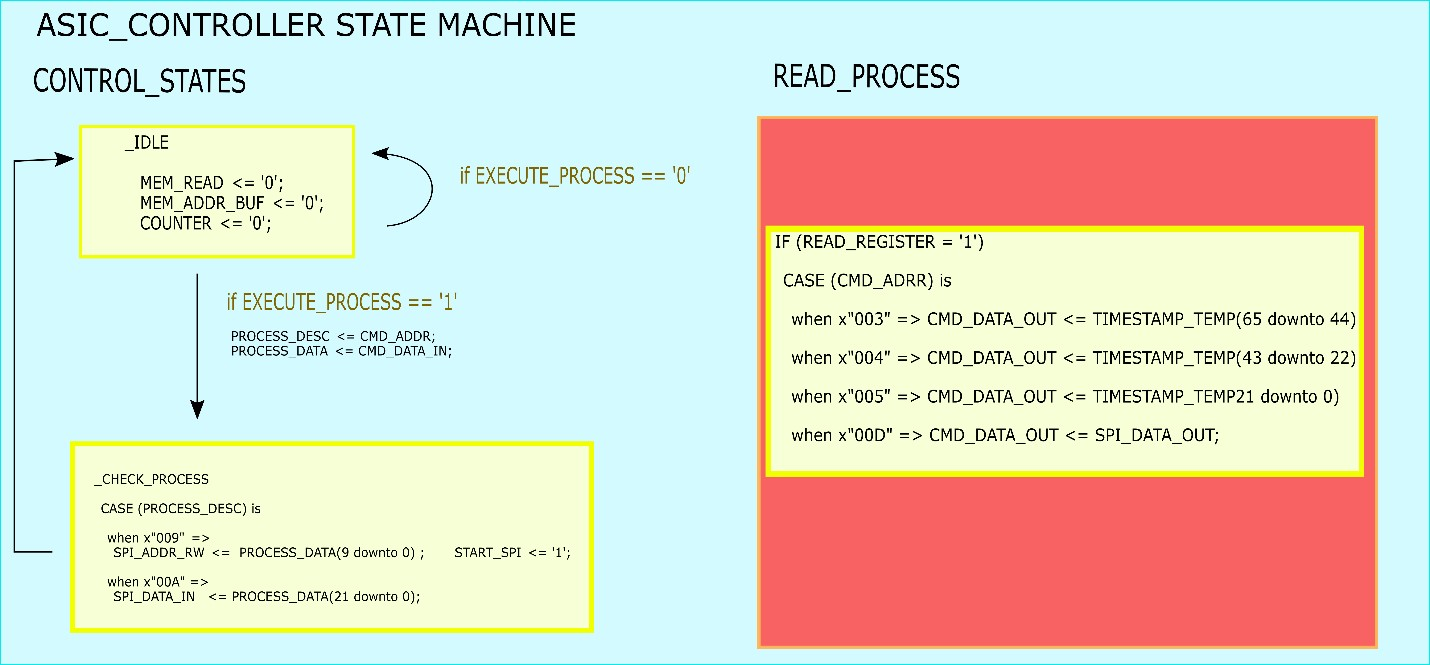
\includegraphics[width=0.89\textwidth]{ASIC_Controller_STATEMACHINE.jpg}
    \caption[]{ASIC Controller State Machine}
    \label{fig:ASIC_CON_STATE}
\end{figure}

After the System Controller has parsed the input, it will either send an impulse on the EXECUTE\_PROCESS or the READ\_REGISTER line, the former defines the data or the address of the registers of the ASIC that should be read or written through the CMD\_ADDR and CMD\_DATA\_IN registers.

One hierarchy stage below, the SPI Control Unit is affiliated in the design. The SPI Control Unit is in turn one stage above the SPI-Master and is mainly responsible for implementing system resets for the SPI port that are sent from anywhere in the command processing unit, it can overwrite the SPI clock and the data lines if a reset is requested. Its state machine diagram can be found below. 

\begin{figure}[H]
    \centering
    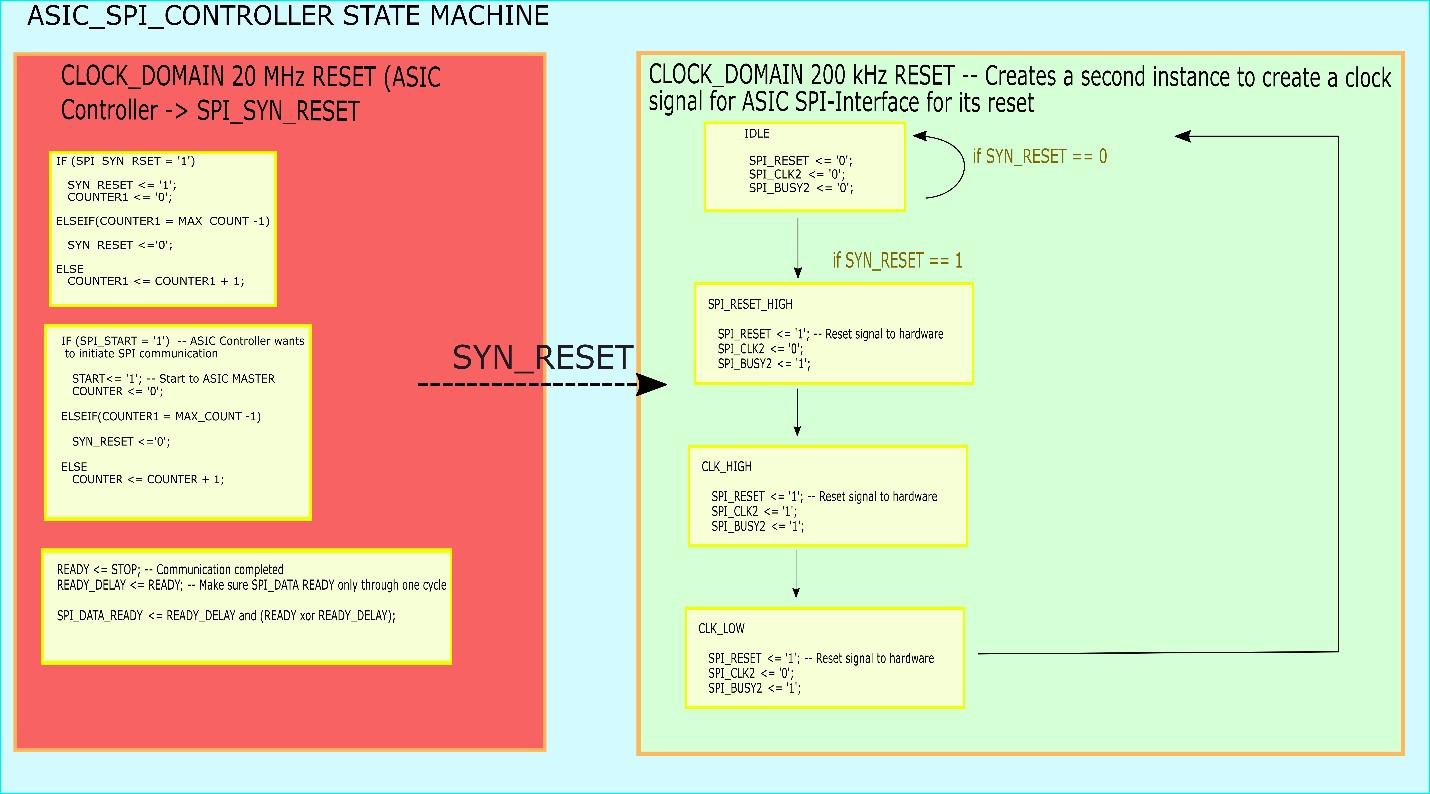
\includegraphics[width=0.8\textwidth]{SPI_control.jpg}
    \caption[]{SPI Control Unit State machine, clock domains and non-sequential logic part}
    \label{fig:ASIC_SPI_STATE}
\end{figure}

And finally, the SPI Master is added one stage below whose outputs and inputs are directly connected to the digital hardware interface of the ASIC. The SPI master combines the SPI-Address the Read/Write Mask bit and the SPI-Data to a 32-bit register which is serially transmitted over the SPI interface if the ASIC Controller initiates an SPI transaction. The state machine of the SPI-Master is depicted in the figure below.

\begin{figure}[H]
    \centering
    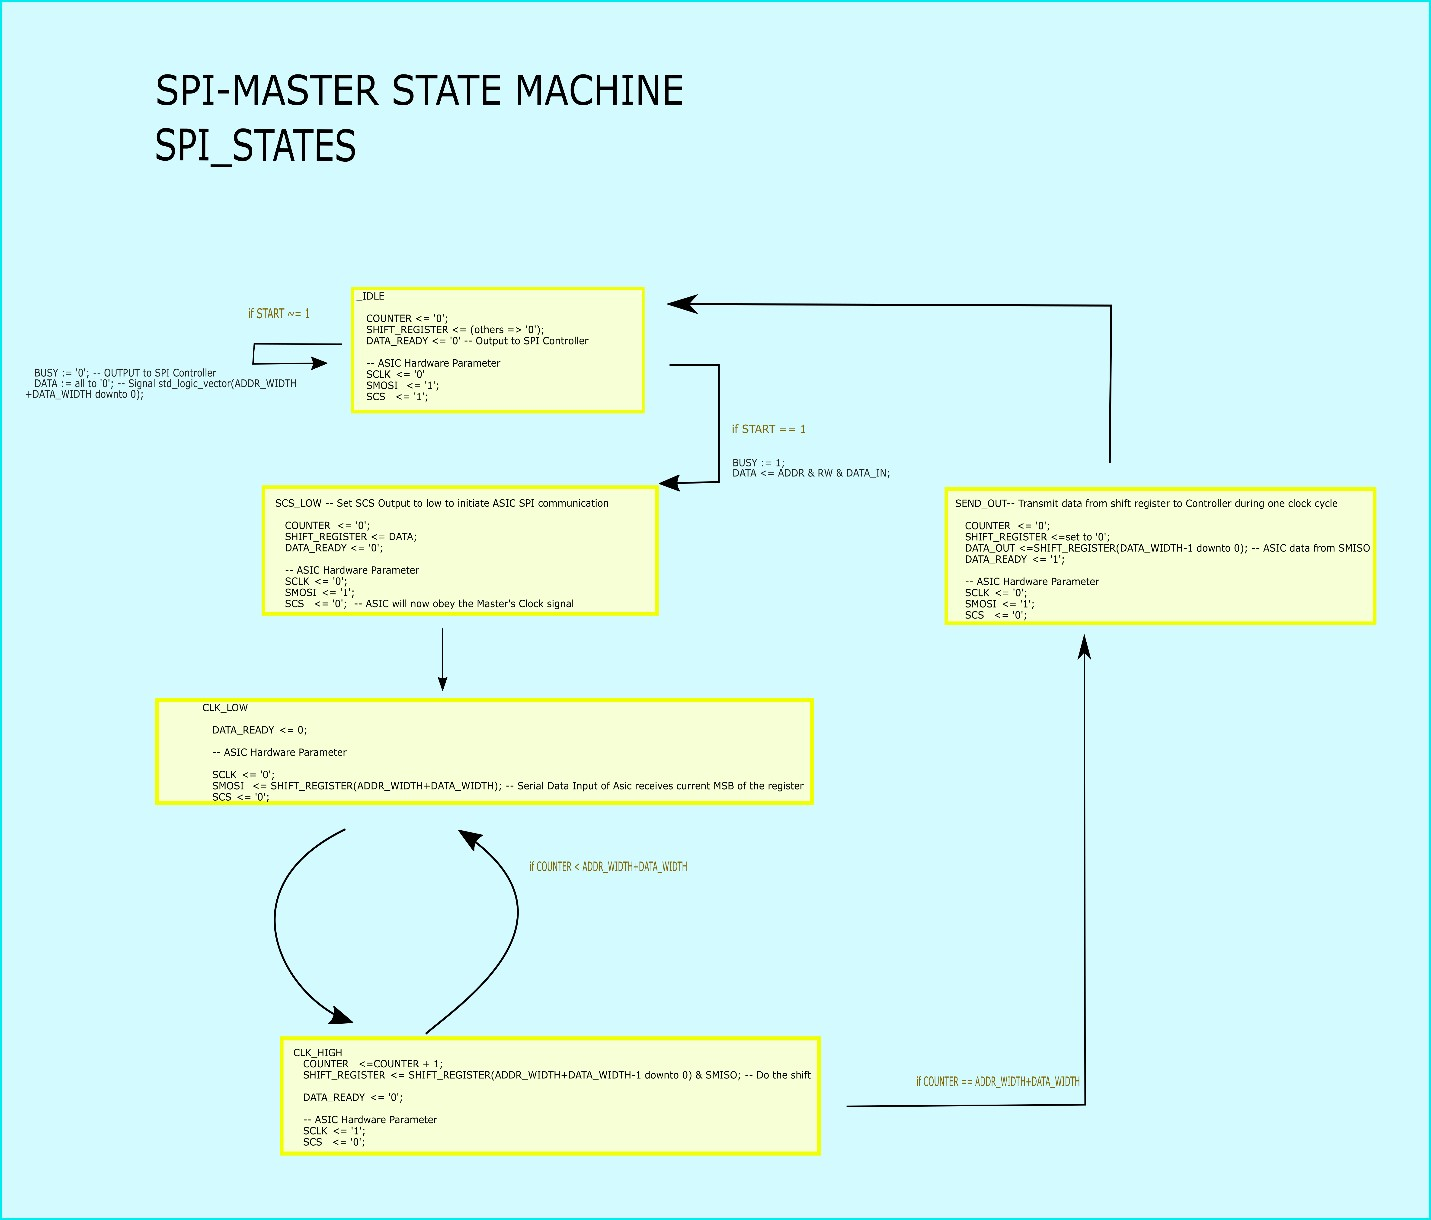
\includegraphics[width=0.8\textwidth]{SPI_master.jpg}
    \caption[]{SPI-Master State Machine}
    \label{fig:SPI_master}
\end{figure}




 \newpage
\section{Systems Engineering Considerations}
\label{sec:systems_engineering}

\subsection{Power Budget of the Readout Electronics}
\label{sec:power_budget}
This power budget (see tab. \ref{tab:power_budget}) is based on the power consumption in the data sheets of the electronic components used in the design.
The power consumption of the FPGA is a large estimate, since it depends on the implemented logic.
Also the DRS's power consumption is an estimate based on the value given in a book\footnote{Typical specifications for pixel chips used in particle physics: Power dissipation per pixel \textless $50\mu m$.\cite{rossi2006pixel}}, the real value will depend on the final design.
\begin{table}[H]
	\centering
    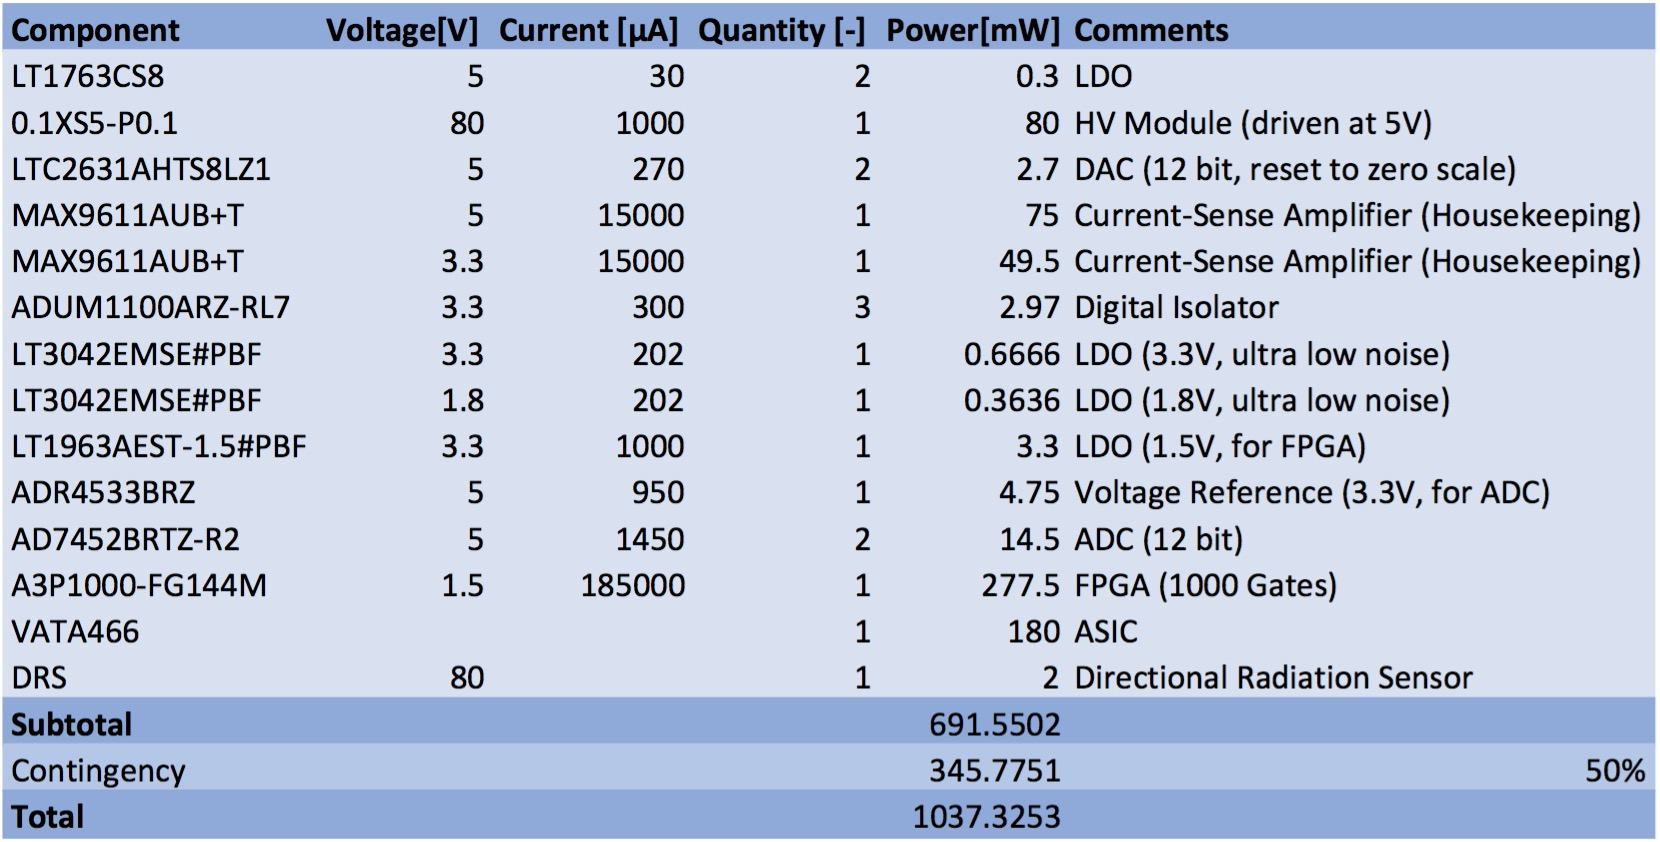
\includegraphics[width=1\textwidth]{power_budget.jpg}
    \caption[Power Budget]{Power budget of the DRS electronics.}
	\label{tab:power_budget}
\end{table}

The budget seems to be realistic, since the total consumed power is close to the 0.9W\cite[p. 11, tab. 4]{tantalumproject2016} of the RADEM mission, which uses a similar DRS.

\subsection{\texorpdfstring{$I^2C$}{TEXT} Interfaces}
\label{sec:i2c_interfaces}
Some electric components in the design can only be accessed via an $I^2C$ interface. 
Their addresses are defined in the following table:
\begin{table}[H]
	\centering
    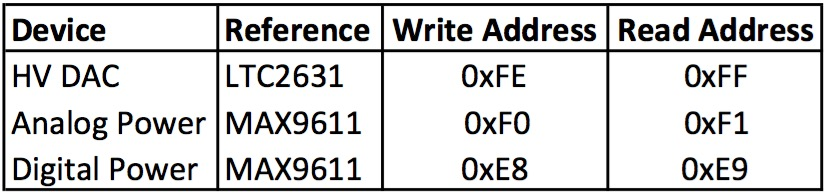
\includegraphics[width=0.5\textwidth]{i2c_interfaces.jpg}
    \caption[$I^2C$ Interfaces]{$I^2C$ interface addresses.}
	\label{tab:i2c_interfaces}
\end{table}
 \newpage
\section{Conclusion}
\label{sec:conclusion}
The project accomplished a first electronic and logic design to readout the DRS from PSI for the Tantalum cubesat mission.
The vast information gathered should help a future student to quickly catch on to the task and thereby help her or him to improve and extent the existing work.
The next important step in development is the exact system engineering level decision on a data bus architecture inside the cubesat.
A PCB would need to be produced to test the DRS's readout electronics, during this process more profound trade-offs would need to be done considering the footprint of the components.
%TODO For the logic part blabla, do more shit, blablabla

We learned a lot of interesting and new concepts during this project.
It also let us experience the difficulties in the design of a payload instrument.
Numerous parameters have to be traded off and the many interdependencies with other subsystems and organizations made this task a fascinating challenge.

The Tantalum mission aims to study a still unknown world just outside of the Earth's atmosphere.
It's potential outcome would have a huge impact on commercial, as well as scientific satellites and would enable a wider use of new propulsion technology, like electric propulsion.
We hope that this contribution will bring the project a step closer to realization and launch.

%Data rates and digital resources need to be re-evaluated every time the design is updated and expanded.
 \newpage

\newpage
\nocite{*}
\bibliography{report.bib}{}
\bibliographystyle{abbrv}

\newpage
\appendix
\section{Schematics}
\label{sec:schematics}
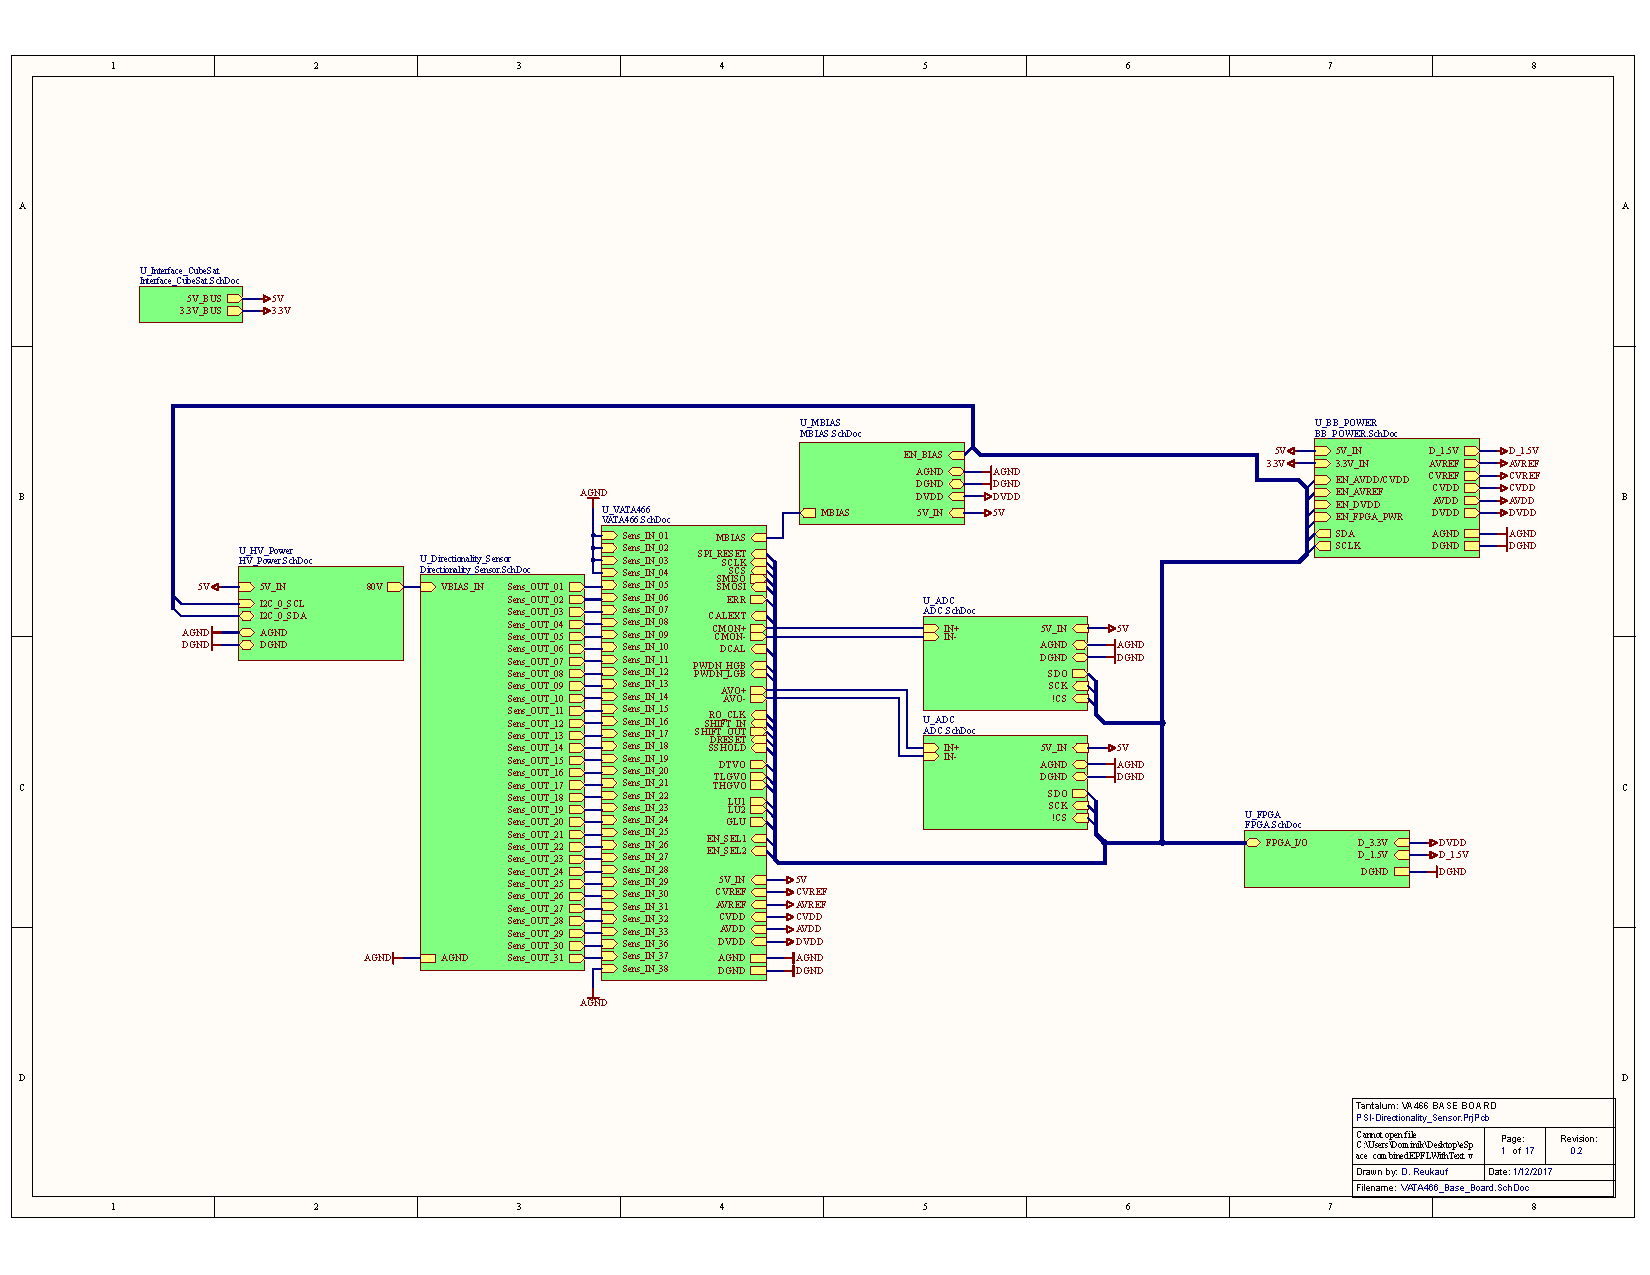
\includepdf[landscape=true,pages={1-17}]{PSI-Directionality_Sensor.pdf}
\newpage

\section{VHDL files}
\label{sec:VHDL}


\end{document}
